% SIXTH DRAFT — editorial refinement of v5, 6 November 2026.
% Task 4 measurements and the submission freeze remain OPEN.
% Evidence comes from the experiment RESULTS files, not earlier prose.
% Nine included figures; group, market, and advertising floats are not included.
% Build: tectonic main.tex
\documentclass[sigconf, nonacm]{acmart}
\settopmatter{printfolios=true}
\AtBeginDocument{\addtolength{\footskip}{36pt}}
\usepackage{enumitem}
\usepackage{microtype}
\usepackage{listings}
\usepackage{graphicx}
\usepackage{xcolor}
\setlength{\emergencystretch}{2em}
\newcommand{\artifactbase}{https://github.com/jacoby149/web10}
\newcommand{\artifactrev}{317fa349eae714ddde07f249ca65cdaa34b6459b}
\newcommand{\artifactdir}[2]{\href{\artifactbase/tree/\artifactrev/#1}{#2}}
\newcommand{\domainartifactrev}{26720acba859c7eb03fc5d26a6221cdde5b764a1}
\newcommand{\evidence}[2]{\href{\artifactbase/tree/\domainartifactrev/#1}{#2}}
\lstdefinestyle{sql}{language={},basicstyle=\ttfamily\footnotesize,
  breaklines=true,frame=single,framesep=4pt,rulecolor=\color{gray!50},
  backgroundcolor=\color{gray!6}}
\setcopyright{none}
\acmConference[SIGMOD 2027 Industry Track]{SIGMOD 2027 Industry Track}{}{}
\acmPrice{}
\acmISBN{}
\acmDOI{}
\title{Your Data, Your Rules: \\ Extending the Decentralized Web}
\author{Jacob Hoffman}
\affiliation{\institution{web10 Inc.}\country{}}
\email{jacob@web10.app}
\begin{document}

\begin{abstract}
Owning a copy of your posts is not the same as controlling the
relationships around them. \textbf{web10} combines user-managed access
and application-defined computation on one shared columnar store.
Applications submit queries; the node supplies authorized relations
before joins and aggregates execute. Solid composes across pods or an
additional index; a custom AT Protocol view requires an application-owned
sync, database, and serving backend. web10 instead pools authors in
ClickHouse: millions is a sizing target, not measured capacity.
The deployed social application supplies profiles that a game and a
marketplace reuse without a new data backend. Isolated prototypes exercise
foreign-principal authorization and domain-follow continuity after provider
loss. In one historical 1,000-group trial, batching reduced median handler
time from 7.64\,s to 363\,ms, but cost more at one group. Independent repeats,
a paired same-engine authorization baseline, and concurrent full-feed
measurements remain open.
\end{abstract}
\maketitle

\section{Owning the content is not enough}
\label{sec:intro}

What makes your data worth owning is not just the content. It is the
graph around it: who follows you, who belongs to your groups, and who
you have allowed to read or change what. A creator can download a
catalog and still lose the audience that made it valuable. A user can
export a profile and still need the next application to rebuild the
relationships and permissions around it. Ownership needs to reach the
operations performed on the data, not stop at an export file.

The decentralized web has made substantial progress on this problem.
Solid separates apps from user-controlled pods~\cite{solid2016,solid-protocol2024};
cross-user composition fetches pods or adds an index. web10 pools authors;
millions is sizing, not measured capacity.
Mastodon distributes social activity between servers through
ActivityPub~\cite{activitypub2018}. AT Protocol separates user repositories
from relays and application views, supports provider switching, and lets
applications define new record types~\cite{kleppmann2024,at-statusphere}.
An indexed custom view requires its own sync, database, and serving code;
a fitting existing AppView avoids that construction.
Its permission system also supports granular delegation~\cite{at-permissions}.
The remaining design question is not whether applications can reuse
data. It is \emph{where they can compute over it, under whose access
rules, and with how much new infrastructure}.

Consider a game joining a leaderboard to existing social profiles.
Fetching reusable records does not supply a queryable cross-user view.
Instead of building a synchronized index and read API, the application
submits its join to web10's storage node. Each service resolves to the
relations this reader may access. The application needs the data
convention and grants, not a new indexing backend.

\textbf{web10} is a deployed data platform built around that division of
labor. Its node exposes generic document reads and writes, identity and
access configuration, a constrained query interface, and media delivery.
It has no feed endpoint and no platform-owned posts schema. Applications
name their own services and write their own queries. Users manage the
grants as rows in the same database that holds the content. The platform
enforces which relations a query can read; the application developer
chooses and tunes the computation over them. This division describes the
query path, not a completed audit of every node feature: ad preparation
and Discover retain node-supplied infrastructure (\S\ref{sec:limitations}).

The design brings together five properties:
\begin{enumerate}[leftmargin=*,nosep]
\item \textbf{Application-independent data.} Posts, profiles, scores,
and listings use one document substrate rather than separate
application-specific node APIs (\S\ref{sec:model}).
\item \textbf{User-managed access.} Groups, roles, and service-scoped
grants express shared access as editable data (\S\ref{sec:model}).
\item \textbf{Authorized composition.} Application-written joins and
aggregates operate on reader-filtered inputs in a shared columnar
engine (\S\ref{sec:query}).
\item \textbf{Cross-node identity.} A serving node can authorize a
foreign principal after home-issuer certification, without creating a
second user account (\S\ref{sec:network}).
\item \textbf{An address distinct from an account.} A compatible client
can follow a creator-controlled domain and resolve its current public
target after a provider change (\S\ref{sec:domain}).
\end{enumerate}

The first three are exercised by the social application, Snake, and
Marketplace. Cross-node access is demonstrated on two isolated nodes
with independent signing keys. Domain subscriptions are demonstrated
in a separate research client; deployed social follows remain
group-based. These are distinct pieces of evidence, reported in
\S\ref{sec:evaluation}, not a claim that the complete network design is
already a production deployment.

Figure~\ref{fig:app-arch} locates feed construction, discovery, face/media
resolution, orchestration, and acting-identity state in the browser.
The SDK transports SQL and a token but adds no authority. The node
authenticates, checks grants, compiles queries, and prepares media URLs.
ClickHouse holds documents and access metadata; object storage supplies
media bytes separately.

\begin{figure*}[t]
\centering
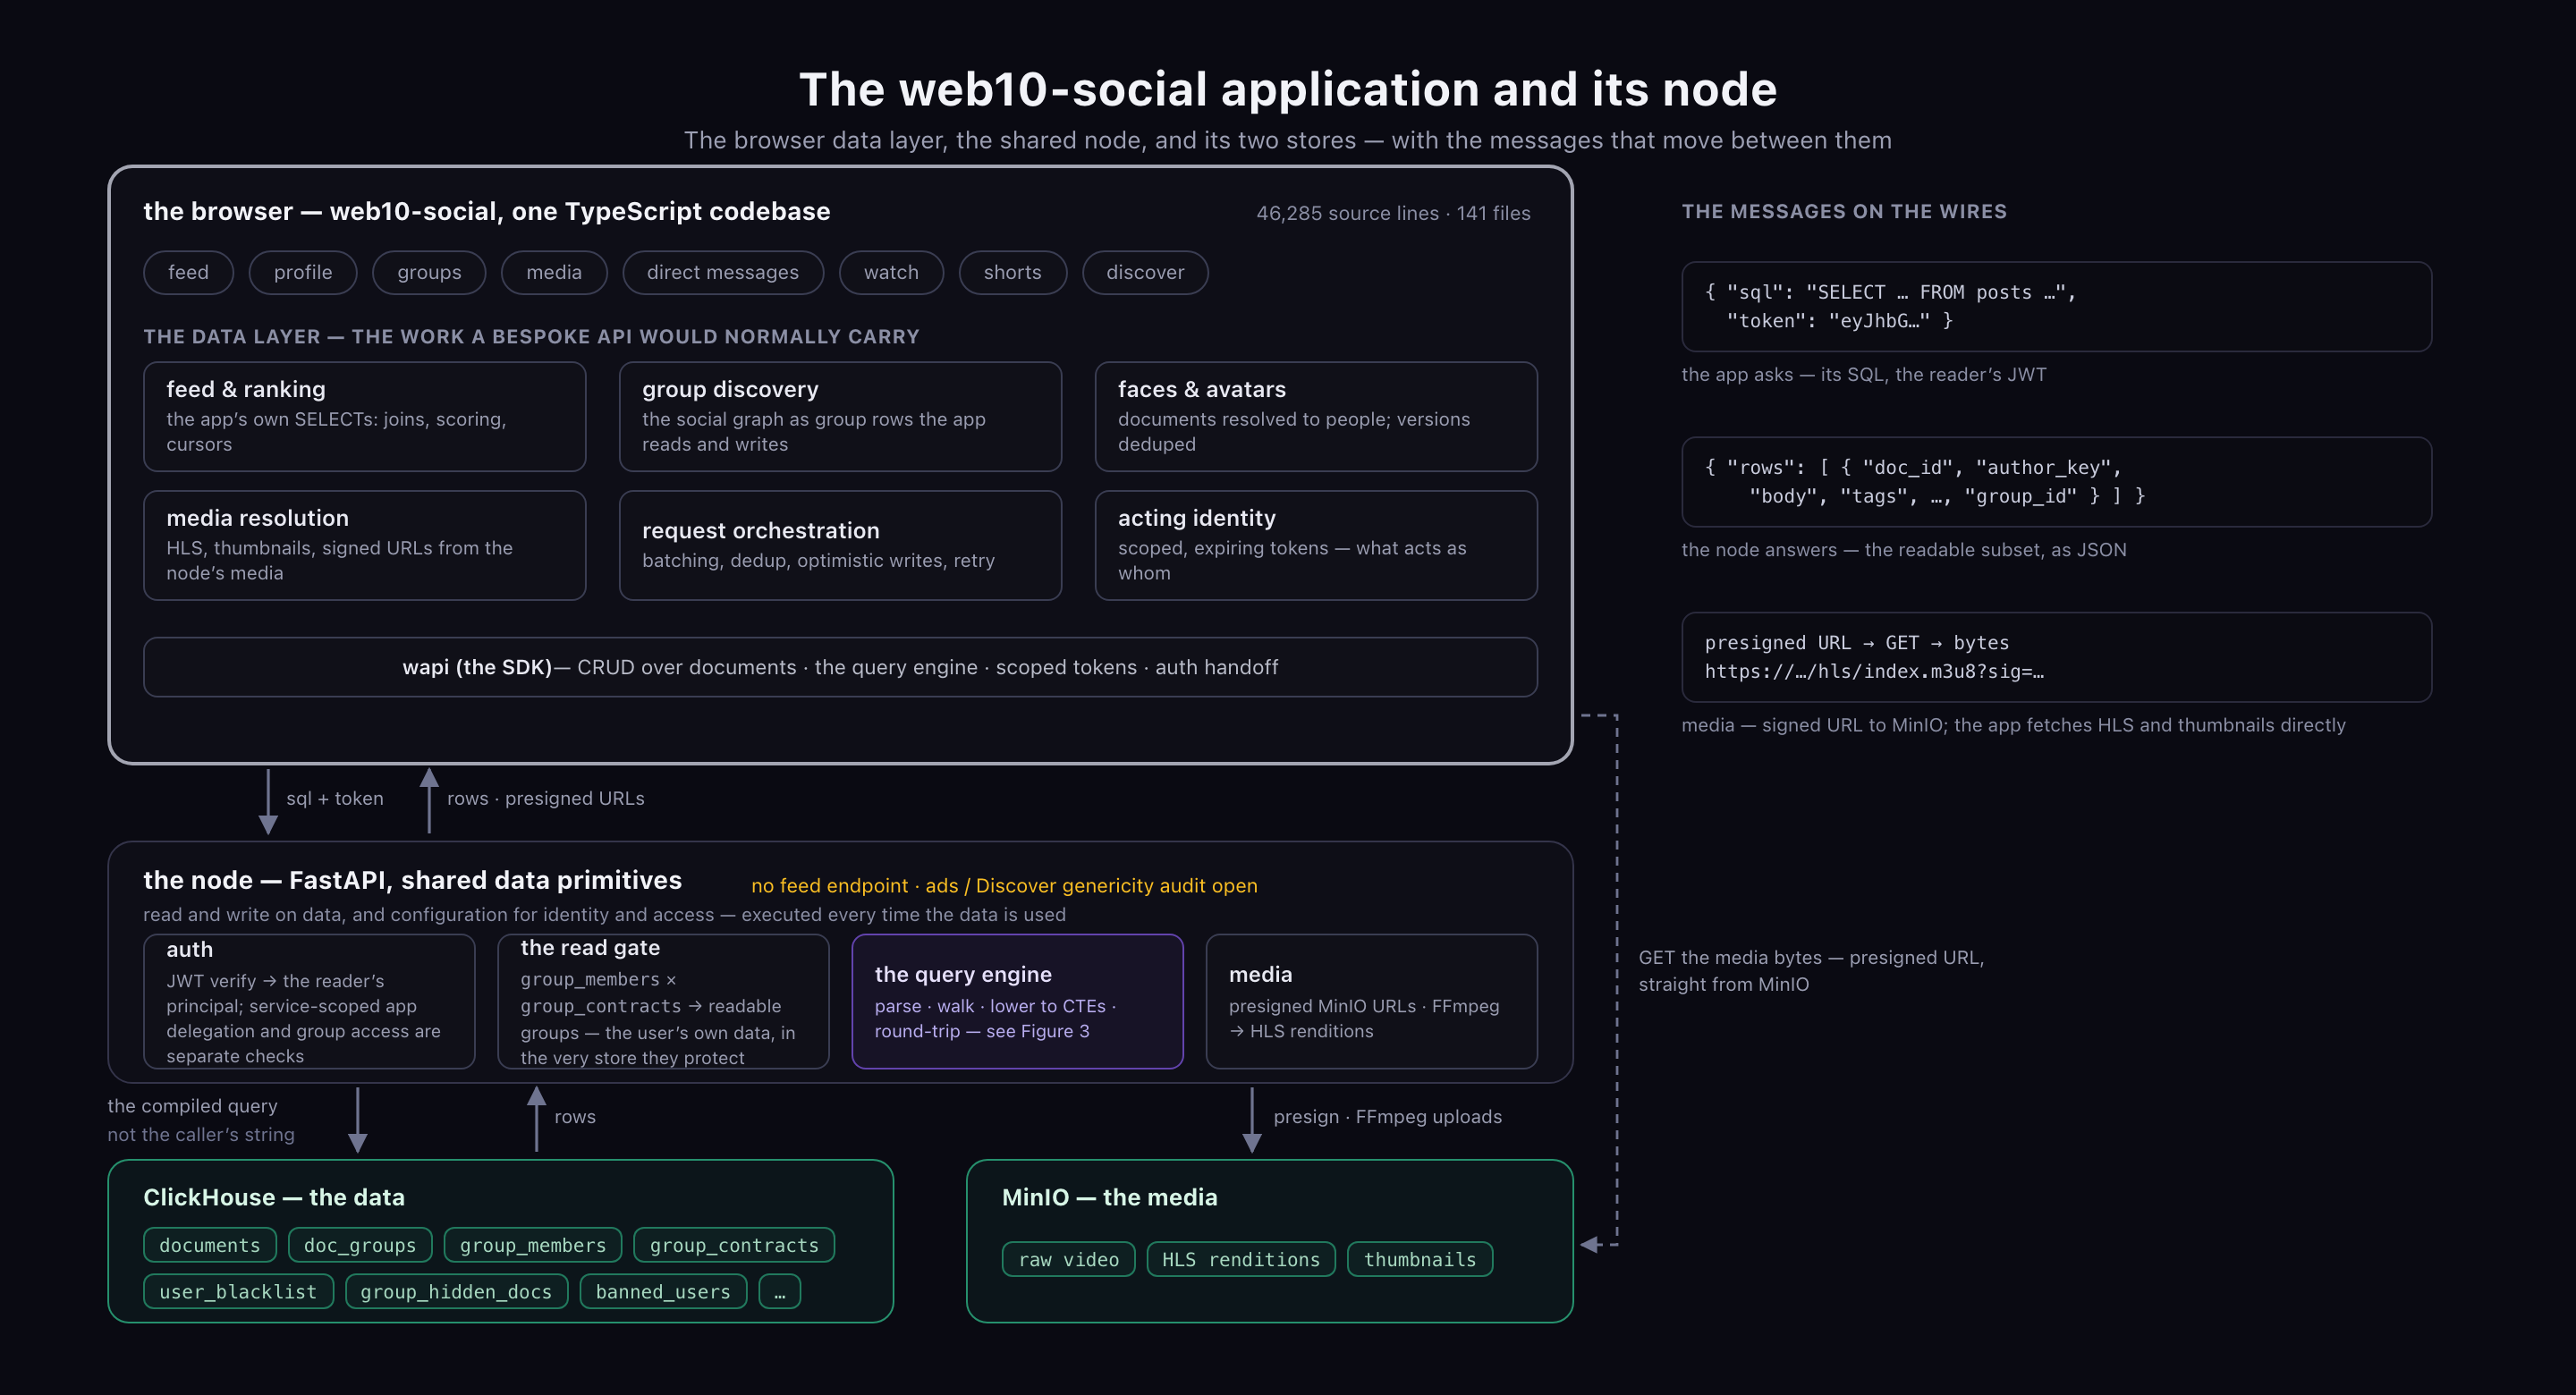
\includegraphics[width=\textwidth]{figs/fig-app-arch.png}
\caption{The application, the generic node, and their message paths.}
\label{fig:app-arch}
\end{figure*}

\section{The rules are data in the store they protect}
\label{sec:model}

A web10 document has an author, an identifier, a service name, and a
JSON body. A post and a game score differ in their service string and
body convention, not in their storage interface. The node never needs
to learn what a score means. Applications agree on the shape of data
they share; the node supplies storage and access, not automatic semantic
interoperability.

Documents attach to groups through \texttt{doc\_groups}. A group contract
defines roles, and \texttt{group\_members} assigns a principal to a role.
A role is a per-service permission map: for example,
\texttt{posts: readAll, create, updateOwn} and
\texttt{comments: readAll}. The reserved principals \texttt{anyone} and
\texttt{authenticated} express access for anonymous and signed-in
readers. A publicly readable group has an \texttt{anyone} read grant.
An invite-only group can therefore remain publicly readable: admission
to membership and permission to read are different decisions.

App contracts express permission for an application to use services;
group membership and class grants express access to content. Revoking
an application's grant does not require leaving a group, and removing a
membership does not require revoking an application. The current content
gate admits active members for reads and creates; non-member reads and
creates use the applicable class grants. Other role-controlled operations
check their named permissions. Thus a role map alone is not the complete
definition of every content decision.

Users manage these relationships through the same API their applications
use. Making a group public writes a grant. Removing access writes a
tombstone. Subsequent checks resolve the current metadata rows. This is
the sense in which the permission model belongs to the user: the user is
the policy administrator for their own hosted data, not merely the
recipient of application-specific sharing buttons.

Both content and metadata live in one ClickHouse database per node.
The \texttt{documents} table is keyed by \texttt{(author\_key, doc\_id)};
the service is stored in \texttt{collection\_name}. A user's namespace is
logical isolation in this shared table, not a physical database per
person. Updates insert newer versions, and deletes insert tombstones.
Reads rank the complete version history before discarding deleted rows.
Discarding tombstones first can expose an older version of a deleted
document or grant.

The node operator can read hosted content. Search, ranking, moderation,
and audit use plaintext, and default end-to-end encryption is not part
of this model. User ownership here means authorship namespaces and
control of application and group grants. Operator conduct is governed
by terms and applicable law; the API does not cryptographically constrain
an operator with physical database access. The design optimizes for
user-controlled data policy and useful computation over it, not
operator-blind storage.

\section{One shared store changes where composition happens}
\label{sec:store}

ClickHouse supplies the analytical engine~\cite{clickhouse2024}; web10
supplies the access boundary around its use. A web10 node pools users in
one shared store, with millions of authors as a sizing target. Discovery,
trending, and ranking can be cross-author queries the application writes
against that store. A leaderboard joins scores to profiles without first
building a synchronized copy of those documents. We have not run a
million-user load test: growing to millions is a ClickHouse sizing choice,
not a change to the composition architecture.

The choice differs from the pod-oriented interface of Solid.
Solid already separates applications from data and supports
user-controlled authorization. It does not require content to be
end-to-end encrypted, and a pod is not necessarily a separate physical
server. The difference relevant here is the exposed unit of composition:
resources reached through pod interfaces versus authorized service
relations queried together inside one columnar engine.

Figure~\ref{fig:composition} locates the fork. In Solid, each user's
resources live behind that user's pod interface. Cross-user discovery
must fetch across those interfaces or use an additional crawler, index,
or query service. Solid can add that infrastructure; pods alone do not
provide a local relational query across users. On web10, the application
queries each selected node's shared store and can merge its results.
One node's local query is not a global network index. The composition
fork holds at any scale; the million-user target is not a capacity result.
Physical colocation brings its own costs:
read-time version resolution, background merges, point lookups on an
analytical engine, and contention between tenants. \S\ref{sec:lessons}
returns to those costs.

The store also needs an application people can use. Solid's social-web
demonstrations establish app/data separation~\cite{solid-demo2016,solid-apps2016};
they do not establish adoption in 2026. Our design choice is not to rely
on unpaid third-party developers to build the primary social application.
We built web10-social alongside the platform, including posts, feeds,
groups, follows, tuning, and monetization. This makes app development part
of the system effort rather than an assumed volunteer contribution.
Its dated operating point and cross-app reuse are evaluated in
\S\ref{sec:evaluation}, not offered as a census of Solid applications.

\begin{figure*}[t]
\centering
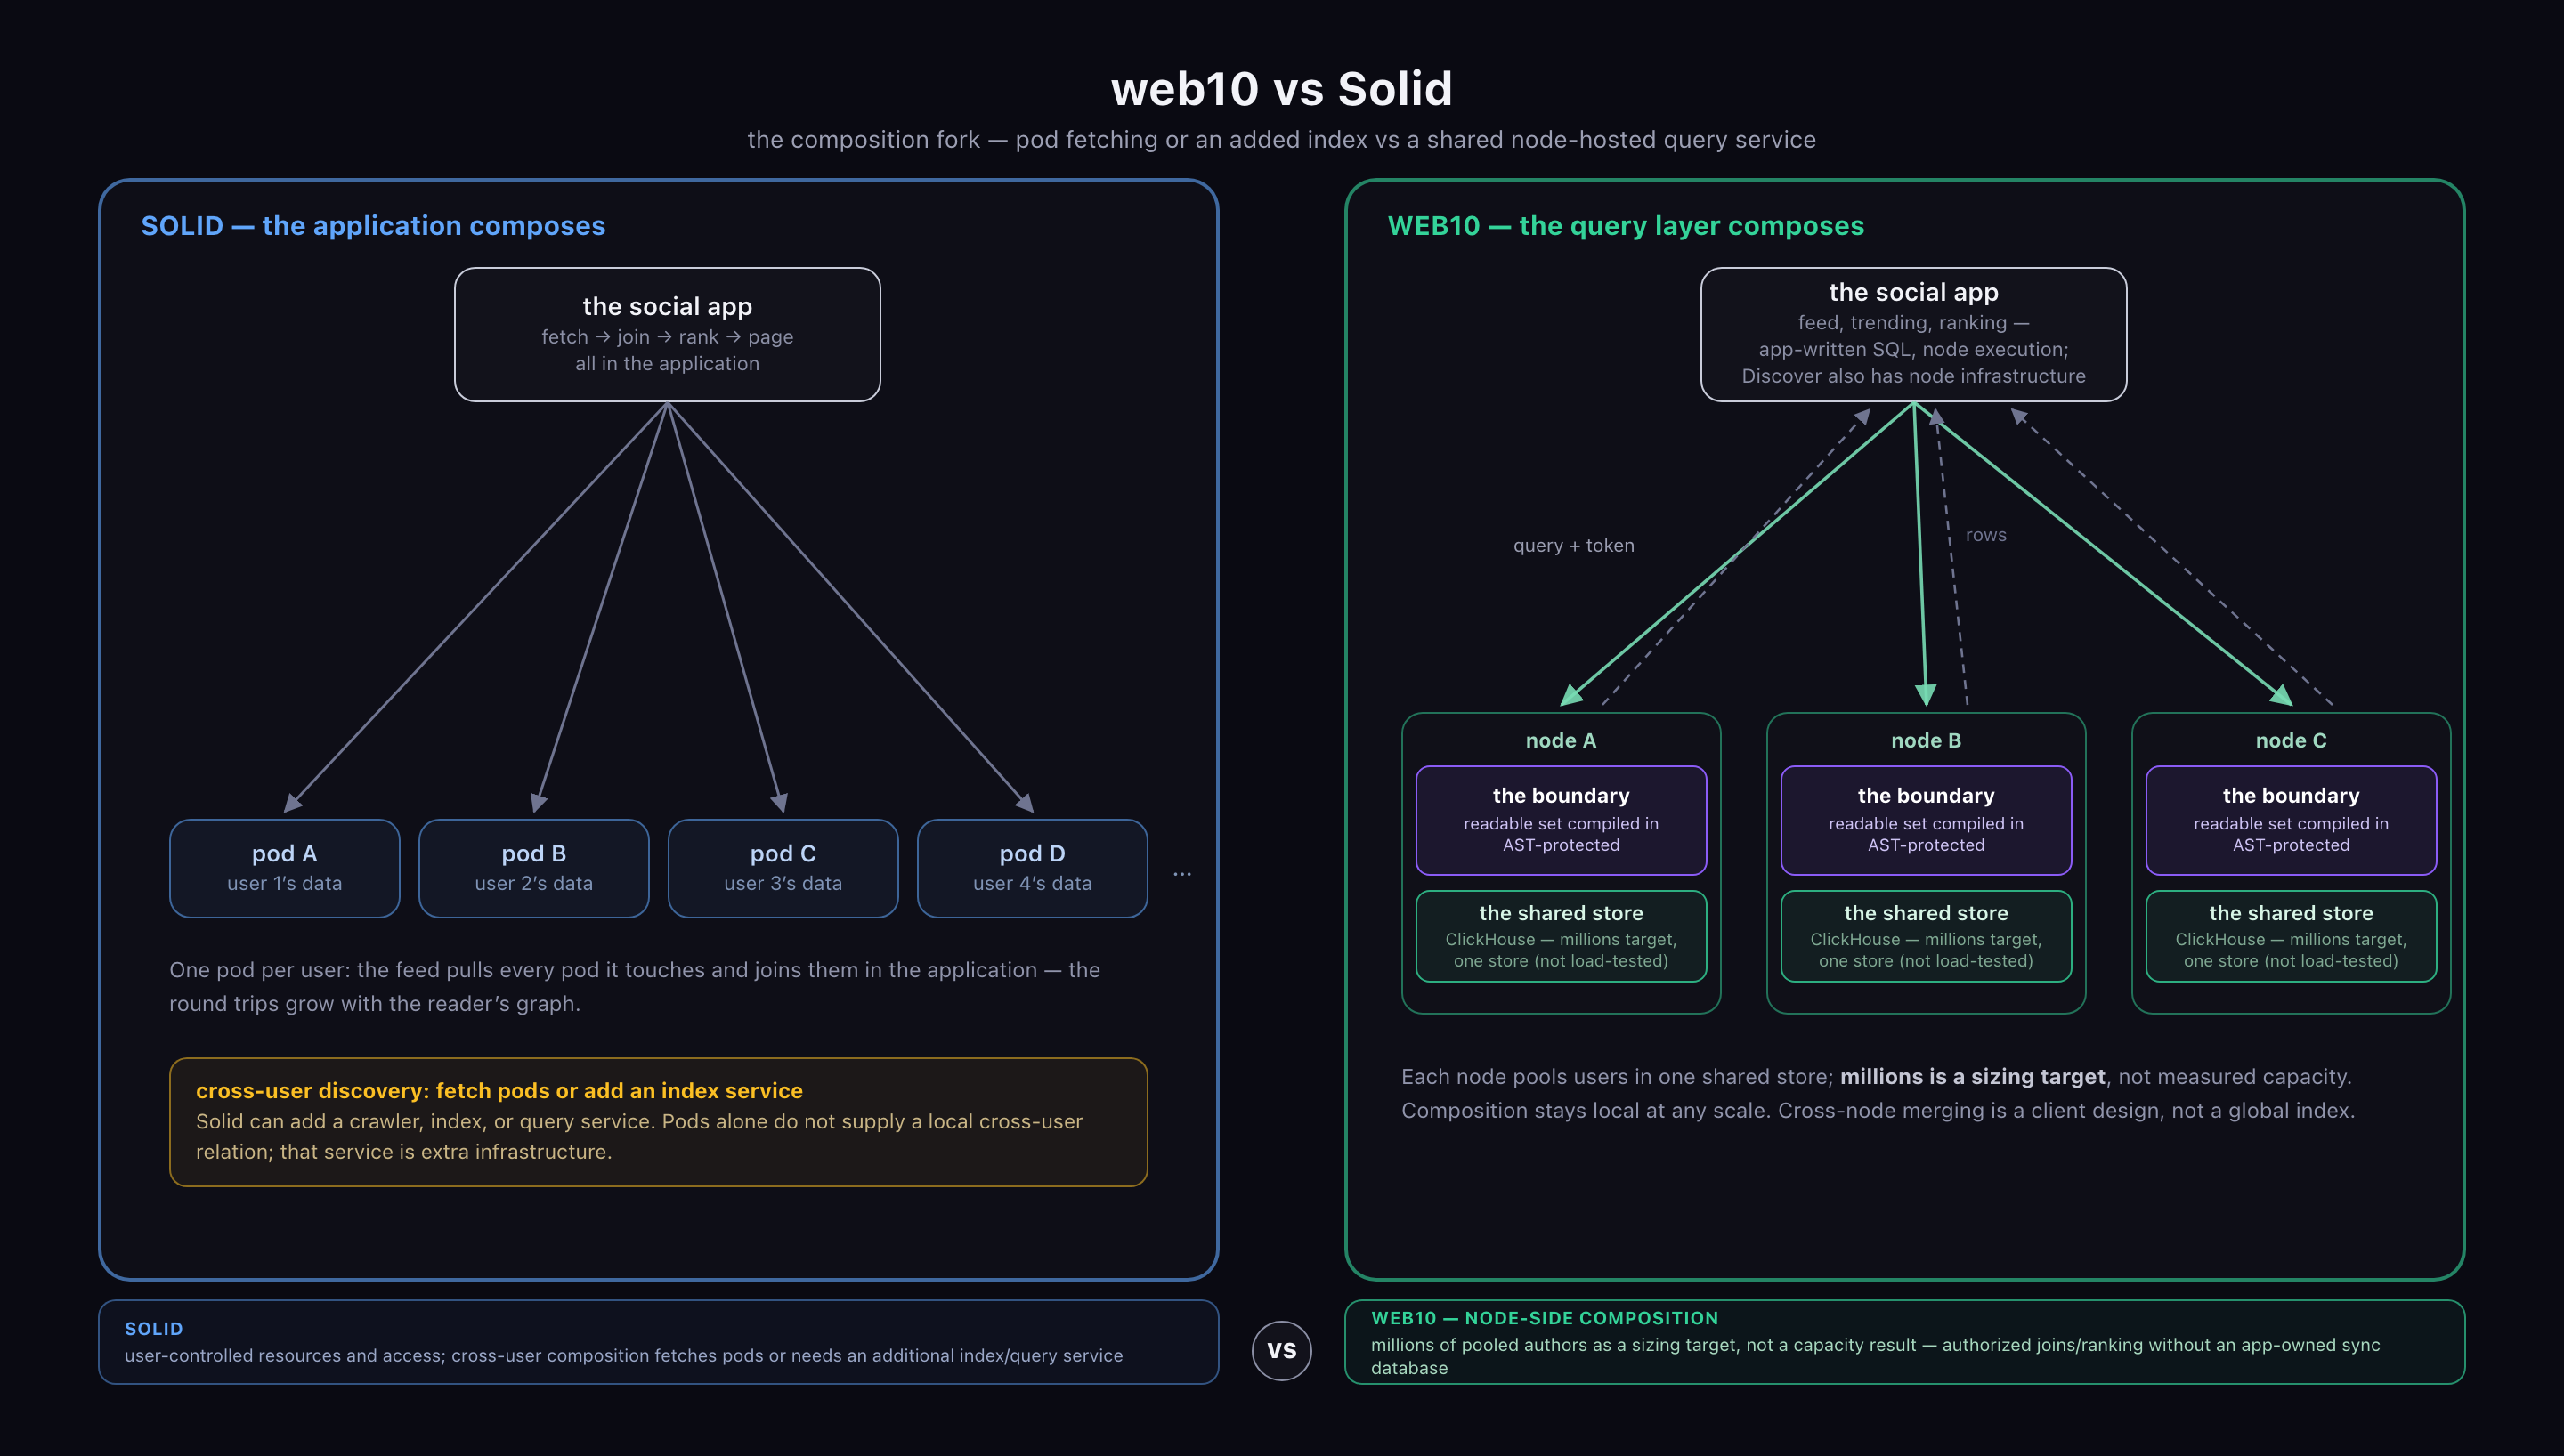
\includegraphics[width=\textwidth]{figs/fig-composition.png}
\caption{web10 vs Solid: shared-node queries and pod composition.}
\label{fig:composition}
\end{figure*}

\section{Your query, over the relations you may read}
\label{sec:query}

An application cannot be allowed to query the raw shared table and then
have its output filtered afterward. Consider this aggregation:
\begin{lstlisting}[style=sql]
SELECT author_key, count(*)
FROM documents WHERE collection_name = 'comments'
GROUP BY author_key
\end{lstlisting}
An outer filter cannot undo counts that already incorporated documents
the reader was not allowed to see. Authorization has to restrict the
inputs to the caller's relational operations.

The application names services: \texttt{posts}, \texttt{reactions},
\texttt{comments}, and \texttt{profile}. Its SDK sends SQL and the token
to \texttt{POST /v3/query}. The node parses the SQL into an abstract
syntax tree (AST) and validates the supported read-only statement shape.
It walks table references inside the query, subqueries, and caller-defined
common table expressions (CTEs). It rejects raw node tables, table
functions, and services outside the applicable application permission.
The caller does not receive a raw database connection.

For each accepted service, the node constructs a \emph{boundary CTE}:
the service's current documents joined to current group attachments,
restricted to groups readable by this principal. Blocks, sharing state,
hidden-document rules, and node bans apply additional exclusions.
The node emits the query from the validated AST and re-parses the result
to require exactly one statement. It executes this generated query,
not the submitted string. Figure~\ref{fig:query-engine} follows the
browser's feed query through these steps.

The consequence is compositional. Each service reference already means
an authorized input relation when the application's joins and aggregates
run. Joining scores to profiles cannot open a private profile merely
because the scores are public. Conversely, granting the application use
of \texttt{profile} does not by itself grant the reader access to every
profile group. The connected controls in \S\ref{sec:ev-interop} exercise
these two gates independently.

This boundary is implemented by the parser, validator, metadata
resolution, generated SQL, and the engine's interpretation of that SQL.
AST construction is not a proof that every possible SQL shape is safe;
parser and engine changes require compatibility and adversarial tests.
The architecture places the access decision on the input relations,
while correctness depends on faithfully implementing that placement.

PostgreSQL row-security policies~\cite{postgres-rls} provide another
placement: the engine applies policies to rows while evaluating queries.
web10 constructs reader-specific relations above the engine, using one
shared database service account. This is a design choice, not a claim
that columnar engines inherently require external enforcement or that
row-level security cannot compose. The intended overhead baseline pairs
web10 enforcement with an equivalent pre-authorized query on the same
ClickHouse engine, data, host, and returned rows/order. It remains unmeasured;
absolute PostgreSQL-versus-ClickHouse latency would confound enforcement
with engine choice.

The developer remains responsible for query performance. The node
provides authorized inputs, not an automatically efficient ranking
algorithm. Resolving those inputs also has a cost of its own. The
fan-out experiment in \S\ref{sec:ev-cost} shows how metadata round trips
can dominate a small document query even when execution in ClickHouse is
fast.

\begin{figure*}[t]
\centering
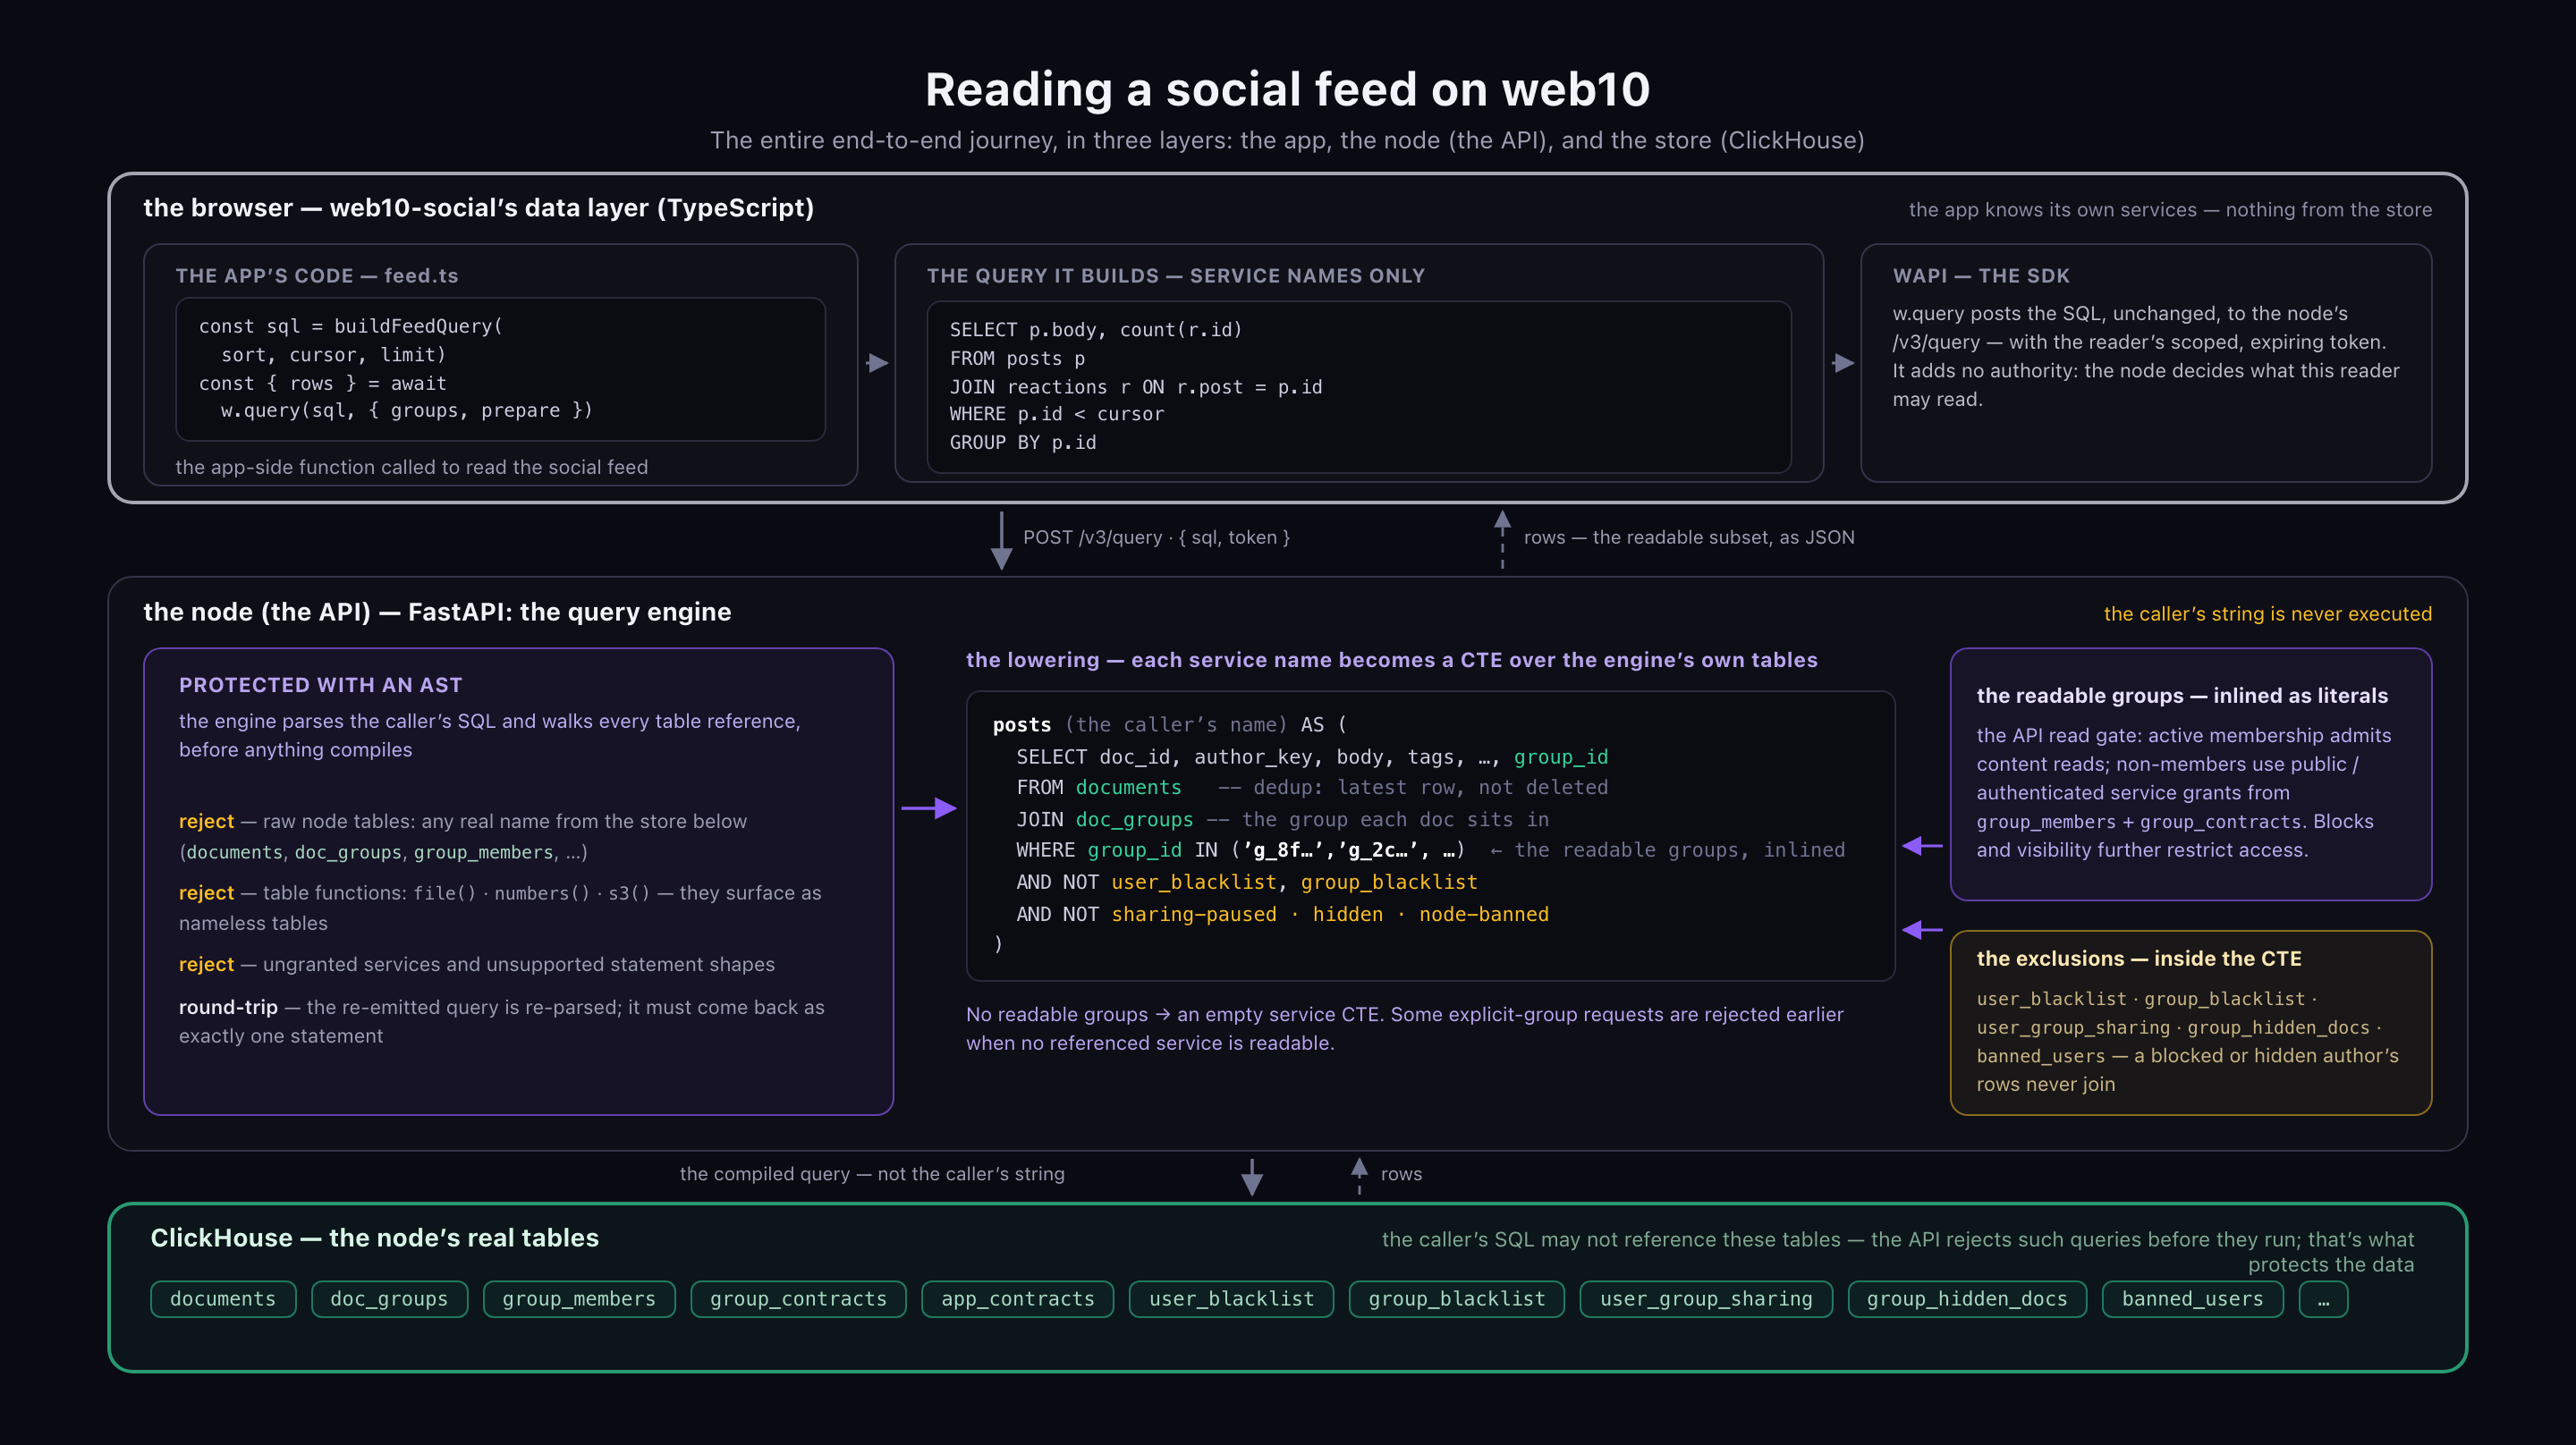
\includegraphics[width=\textwidth]{figs/fig-query-engine.png}
\caption{Reading a social feed: application, query compiler, and store.}
\label{fig:query-engine}
\end{figure*}

\section{A new application without a new data backend}
\label{sec:apps}

web10-social is the platform's primary application and its most demanding
consumer. Text, images, short and long video, audio, groups, and social
relationships share the document, group, query, and media interfaces.
The browser authors feed definitions, power-mean scoring expressions,
joins, ordering, and cursors as SQL; ClickHouse executes them at the node.
This is not browser-side sorting or a node-owned ranking policy. The
\artifactdir{marketing/web10-social/src}{application snapshot} records the
primary consumer. Names, member presentation, and post visibility are
social UI choices expressed through documents and grants. Media objects
reside outside ClickHouse; the
node issues short-lived object URLs and HLS capabilities after the
relevant authorization checks. Capability expiry and document access are
separate lifecycles: removing a grant does not erase downloaded bytes or
instantly invalidate every URL already issued.

Snake and Marketplace exercise reuse rather than another social surface.
Snake writes \texttt{snake\_scores}; Marketplace writes
\texttt{marketplace\_listings}. Both read social-written
\texttt{profile} documents through the user's grants. Their common
dependency is the profile convention, not a new agreement between
application backends. The leaderboard query is ordinary composition:
\begin{minipage}{\columnwidth}
\begin{lstlisting}[style=sql]
WITH latest_profiles AS (
  SELECT author_key, body FROM profile
  QUALIFY row_number() OVER (
    PARTITION BY author_key
    ORDER BY updated_at DESC, created_at DESC,
             doc_id DESC) = 1
)
SELECT s.author_key,
       JSONExtractInt(s.body, 'score') AS score,
       p.body AS profile_body
FROM snake_scores s LEFT JOIN latest_profiles p
  ON s.author_key = p.author_key
ORDER BY score DESC LIMIT 50
\end{lstlisting}
\end{minipage}
Both service names resolve through the query boundary before the join.
An app contract grants use of the required services; group access
determines the readable content. OAuth 2.0 supplies the familiar model
of a user approving an application's delegated access~\cite{oauth2012}.
web10's concrete vocabulary names services, groups, and operations;
OAuth itself does not prescribe how coarse or fine an application's
scope vocabulary must be.

Figure~\ref{fig:mastodon} locates Mastodon's application-data boundary.
Its stock REST API exposes social resources, including profiles
through \texttt{GET /api/v1/accounts/:id}~\cite{mastodon-rest,mastodon-accounts}.
A game or marketplace can reuse those profiles. The illustrated
integration supplies its own score/listing data layer and combines that
data with the profile responses, in application code on the client or
server. web10 supplies storage for all three services and executes their
authorized joins in the node. This comparison concerns the stock
Mastodon interface, not the limits of ActivityPub extensions.

Figure~\ref{fig:atproto} asks a different question: where does a new
cross-user query run? The same social application, game, and marketplace
appear on both sides. AT Protocol does not forbid non-social records:
a developer can define a Lexicon and build an AppView around it. Record
reuse and granular permissions remain available~\cite{at-permissions};
the indexed custom path costs backend work. In the illustrated design,
applications write profiles, scores, and listings to users' repositories.
The application can reuse an existing AppView when its
available data and API provide the required read. Otherwise, it must
design and build its own read backend. The figure draws this fork.
A custom backend does three concrete jobs.
A synchronization process delivers changes to application webhook code
that applies creates, updates, and deletes. A separate application
database holds the selected records in queryable tables. Request-serving
code queries those tables and returns a page or data to the browser.
These responsibilities form an \emph{AppView}-style read backend; they
need not be three separate processes or servers.

The path follows the Statusphere tutorial and its pinned implementation
\cite{at-statusphere,at-statusphere-source}, pinned at
\texttt{dbb97738caa9} (full revision in the cited source).
Statusphere is a social status application. It uses Tap for synchronization,
SQLite \texttt{app.db}, and Next.js with Kysely query functions to serve the page.
Its \texttt{account} and \texttt{status} tables illustrate an
application-designed relational schema. An AppView builder can instead
choose a generic JSON table, separate typed tables, or another layout;
the engine, keys, indexes, and update strategy are implementation choices,
not a storage schema supplied by AT Protocol. The figure's score/profile
and listing/profile joins are illustrative, not Statusphere features.
Existing read services, shared indexes, and direct reads are alternatives
to building that backend. Our protocol design preference is to define
wire format, addressing, and delivery without making developers supply
their own database, sync, indexing, and serving stack. AT's custom-view
route leaves those jobs to the developer in practice, not by mandating a
particular database. A social application may reuse Bluesky's AppView;
a non-social workload that cannot use that view must justify the backend
cost against building an ordinary backend. web10 instead supplies the query API and
authoritative document store at the node. Profiles, scores, and listings
share \texttt{documents}; group/grant metadata have separate node-managed
tables. Applications design JSON conventions and queries, not a new
content table, synchronization copy, or read server. The node checks the
query/token, constructs authorized inputs, executes, and returns rows.
The advantage is supplied infrastructure for
authorized computation, not exclusive extensibility or a measured
performance difference.

The screenshots in Figure~\ref{fig:interop} show the resulting reuse:
one social-written identity appears beside a genuinely earned score and
a marketplace listing. These are direct browser captures with synthetic
accounts. The corresponding consent, revocation, and exact-result
checks are reported in \S\ref{sec:ev-interop}. This establishes reuse,
not a completed genericity audit of the node. Ad preparation attaches
\texttt{ad} and \texttt{node\_ad} from node-side loaders, while group
discovery uses a \texttt{discoverable} flag, directory, and Discover-group
enrollment. These surfaces leave the no-app-specific-node-surface criterion
open (\S\ref{sec:limitations}).

\begin{figure*}[t]
\centering
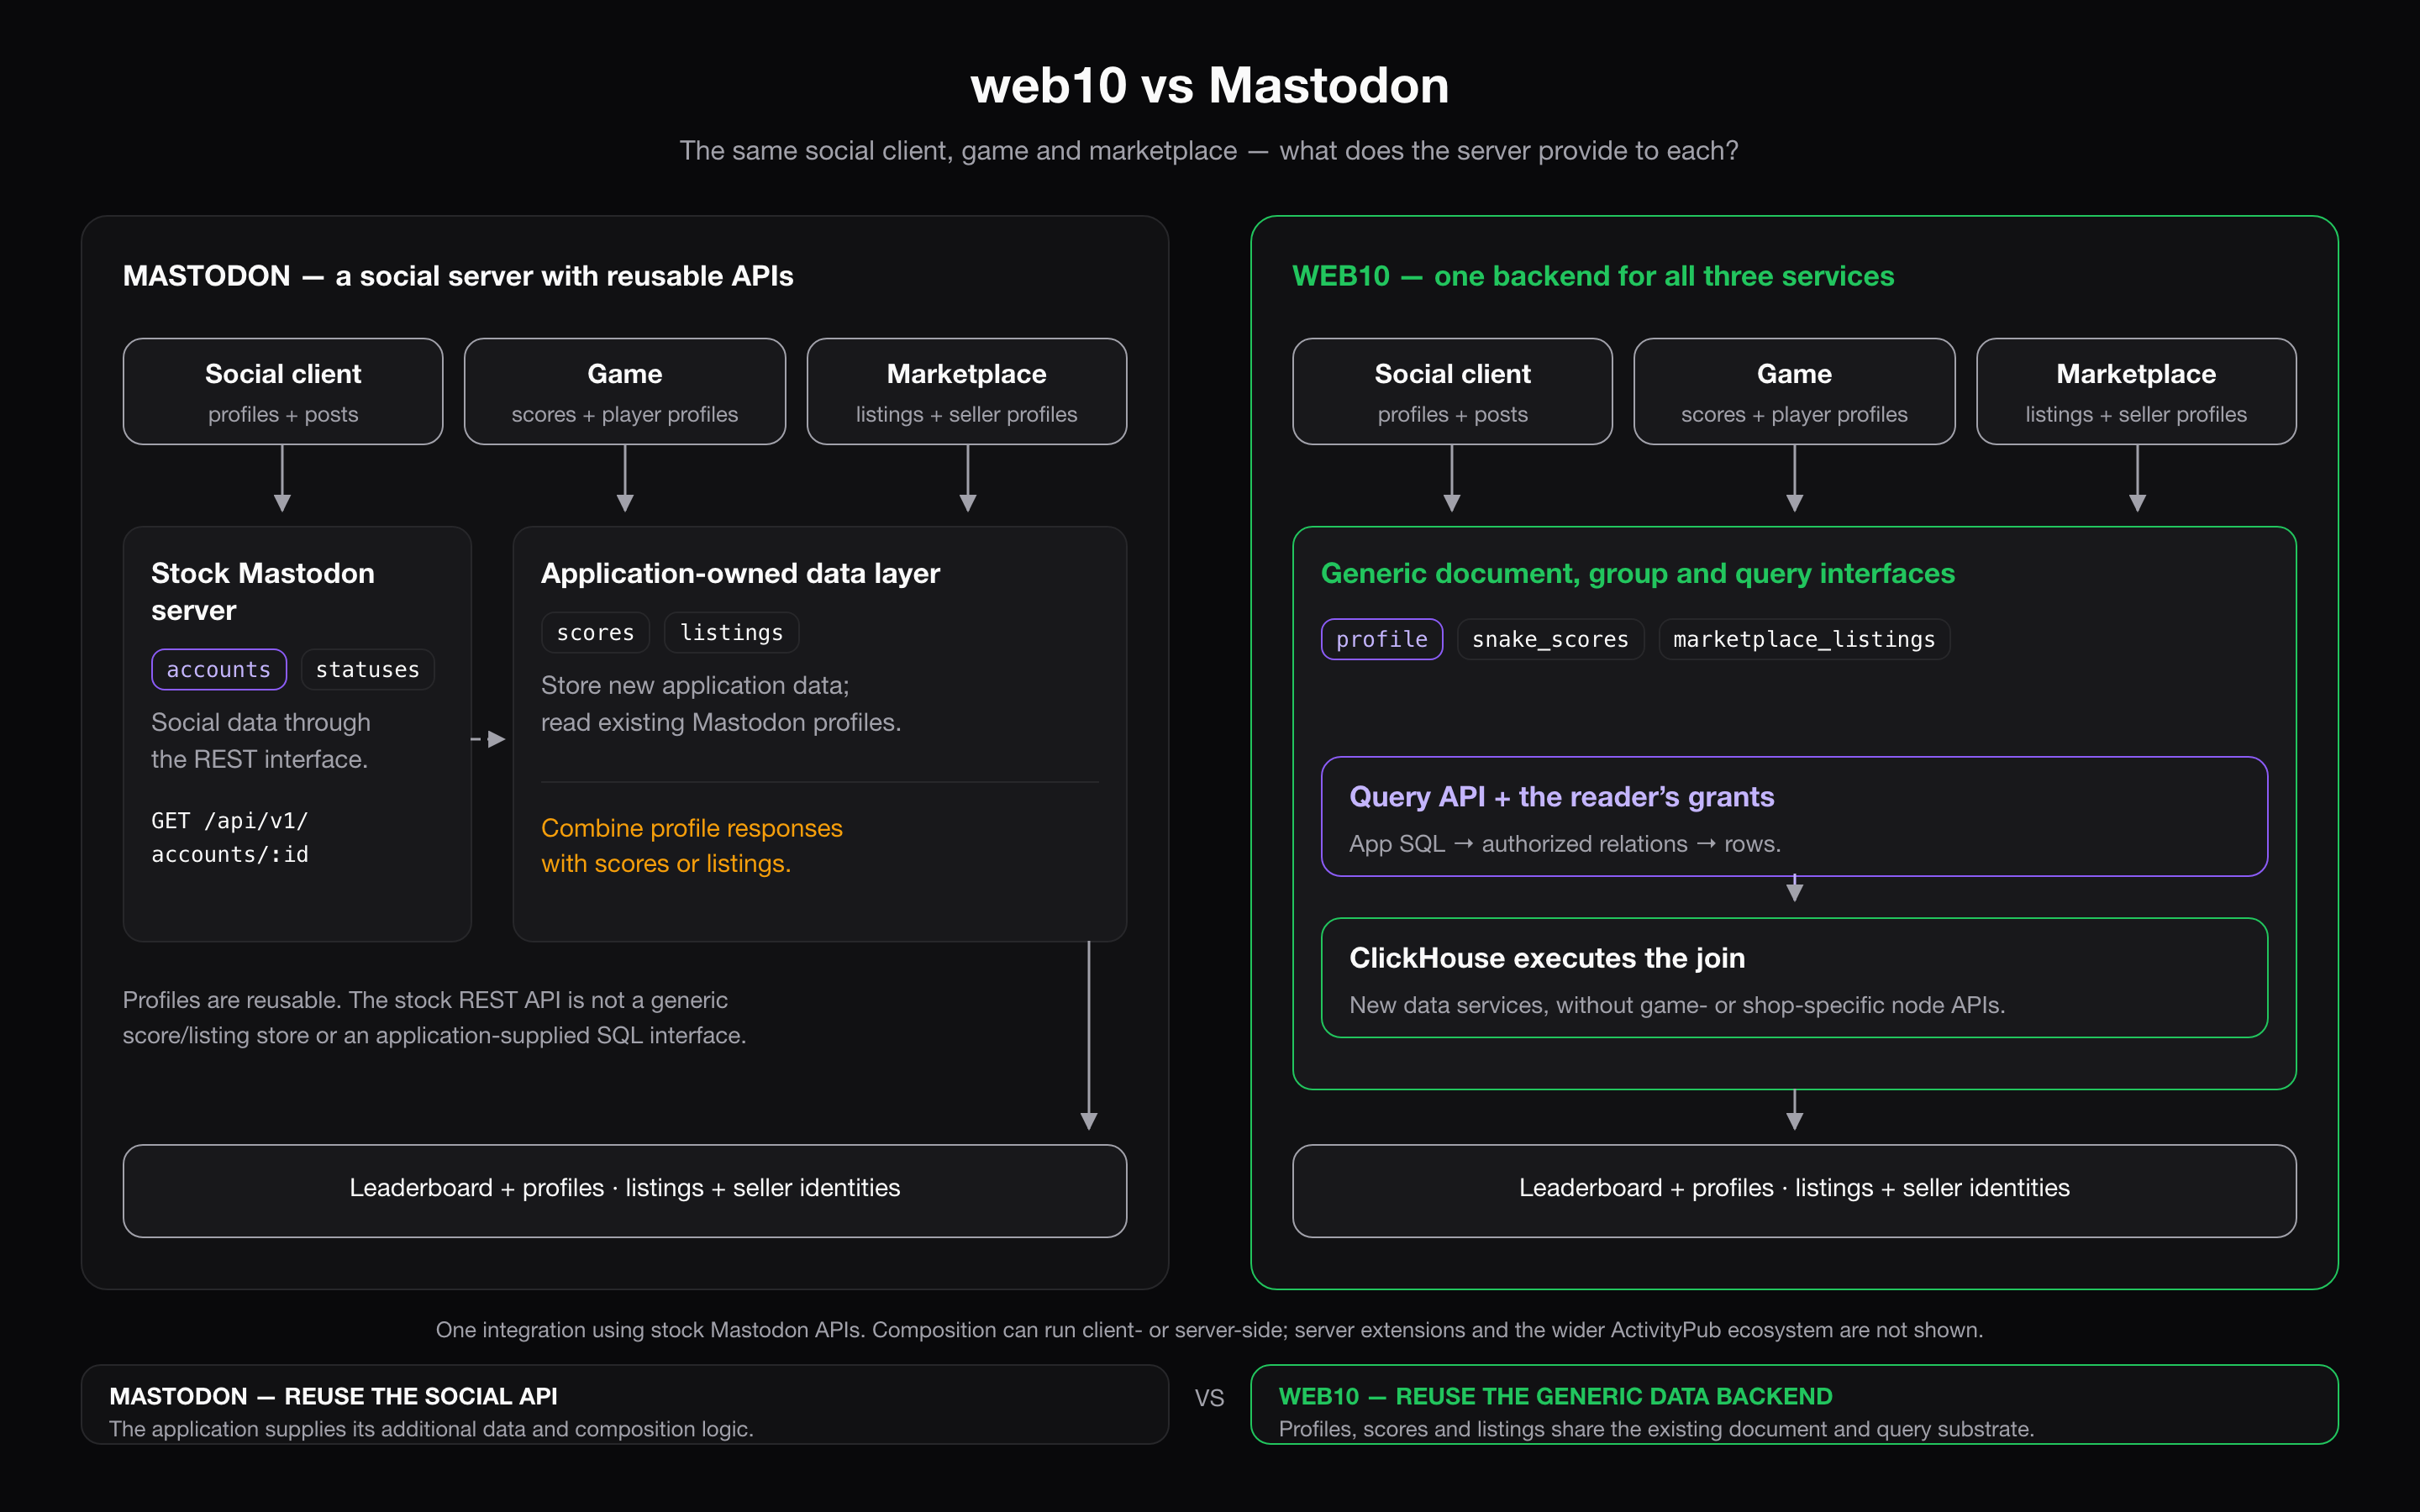
\includegraphics[width=\textwidth]{figs/fig-mastodon.png}
\caption{web10 vs Mastodon: the application-data boundary.}
\label{fig:mastodon}
\end{figure*}
\begin{figure*}[t]
\centering
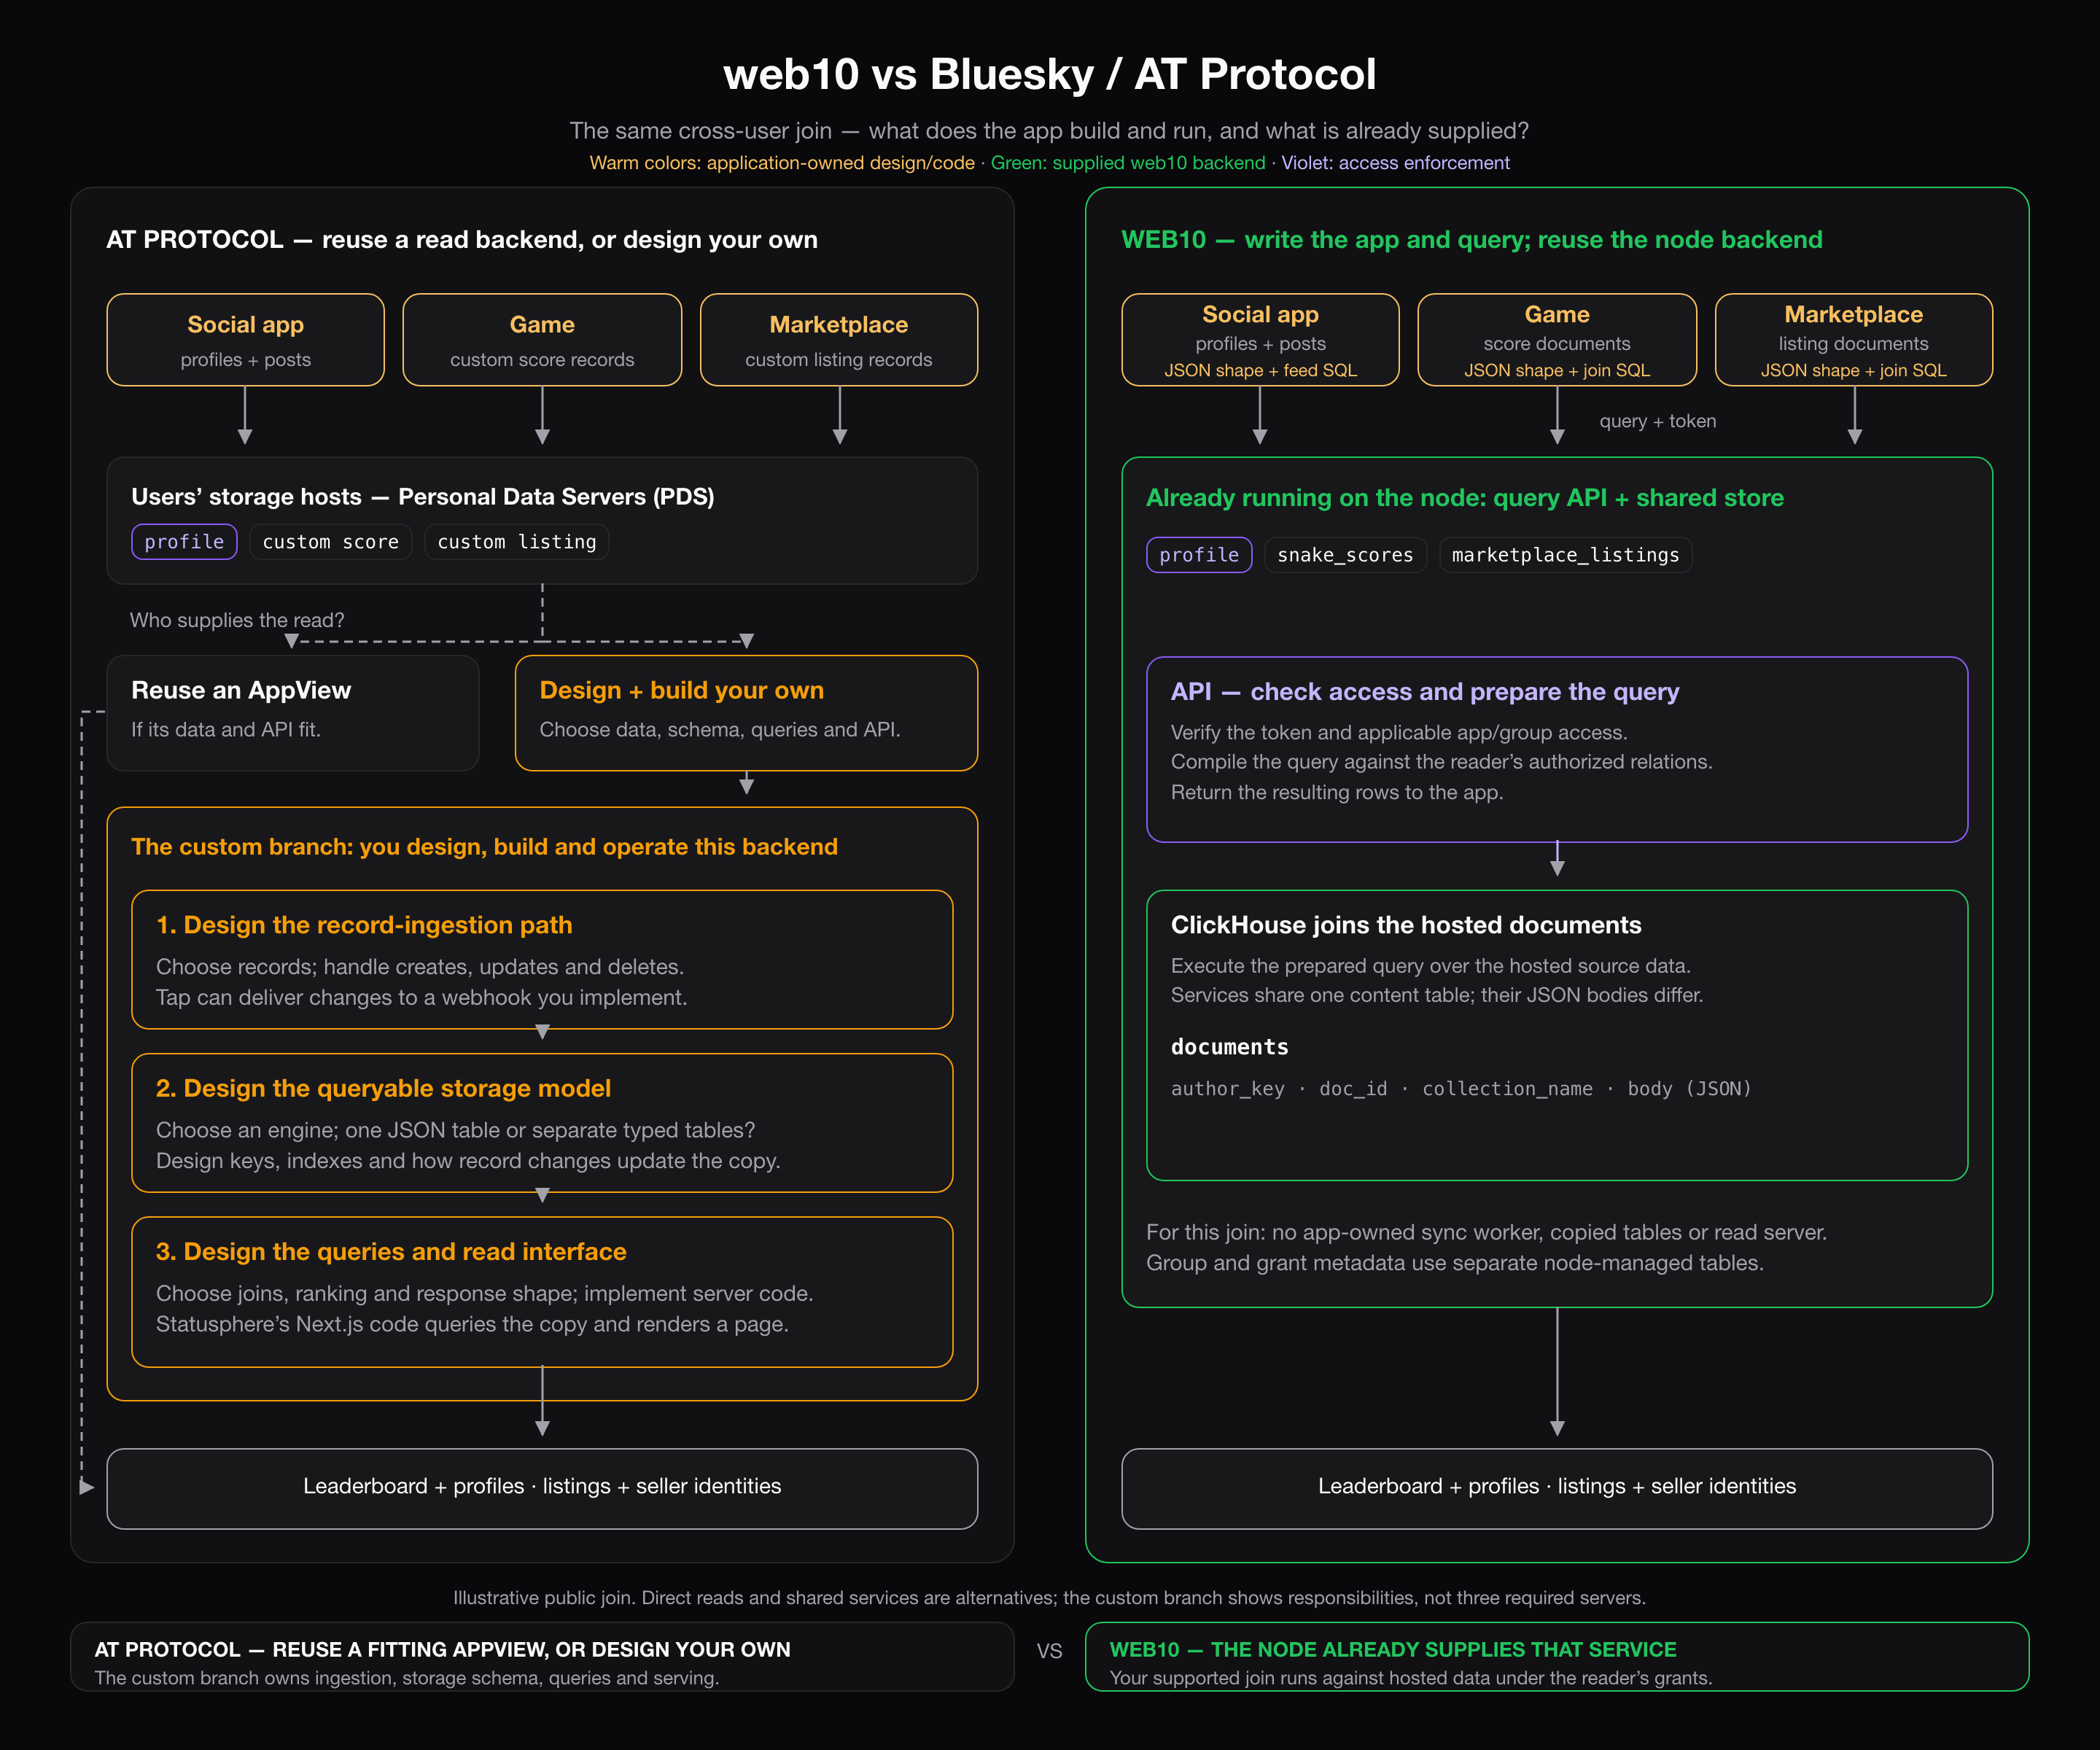
\includegraphics[width=\textwidth]{figs/fig-atproto.png}
\caption{web10 vs Bluesky / AT Protocol: the read backend, unpacked.}
\label{fig:atproto}
\end{figure*}
\begin{figure*}[t]
\centering
\begin{minipage}[t]{0.46\textwidth}
\centering\textbf{Snake: score + social identity}\\[4pt]

\includegraphics[width=\linewidth]{../interoperability-demo/figures/snake-identity.png}
\end{minipage}\hfill
\begin{minipage}[t]{0.46\textwidth}
\centering\textbf{Marketplace: listing + social identity}\\[4pt]
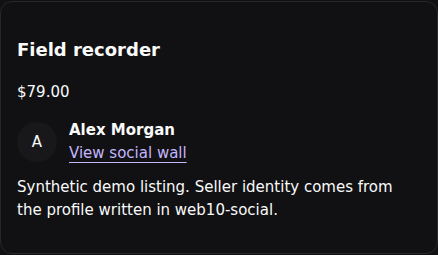
\includegraphics[width=\linewidth]{../interoperability-demo/figures/marketplace-identity.png}
\end{minipage}
\caption{One social-written profile reused by two applications.}
\label{fig:interop}
\end{figure*}

\section{Across nodes: identity is verified, access stays local}
\label{sec:network}

The network design gives a principal a provider-qualified identity:
\texttt{provider/username}. A user has a home account, but a group on
another node can grant that principal access without creating a local
namesake account. The serving node must establish two things separately:
whether the home issuer recognizes the token, and whether this principal
has access under the serving node's own rules.

The \texttt{/certify} exchange answers the first question. The serving
node asks the token's home issuer over HTTPS and caches a successful
answer for that exact JWT until its expiry. The answer verifies identity;
it is not a grant. Each subsequent content read still resolves current
access at the serving node. Email's sender checks offer a useful
analogy: SPF and DKIM establish facts about an arriving message's origin,
not a right to bypass the recipient's rules. The mechanisms differ, but
the separation between verification and authorization is the same.

Figure~\ref{fig:feed} illustrates the intended client-mediated read
model. The client groups its targets by provider, queries the selected
nodes with its home token, and merges independently authorized results.
One node never needs database credentials for another node's store.
ClickHouse's \texttt{remote()} and \texttt{cluster()} are therefore not
the cross-operator interface. A remote API response is content to render
or merge, not SQL to execute locally and not evidence of a local grant.

The two-node experiment demonstrates certification and owner-managed
foreign grants on both document and query reads. Complete client-side
feed merging, foreign enrollment, and independent production-node
provisioning remain integration work. Local paths still use legacy bare
principal keys while the exercised foreign paths use qualified keys;
the coordinated identity migration is not complete. The figure describes
the network arrangement, not a measured production cross-node feed.

\begin{figure*}[t]
\centering
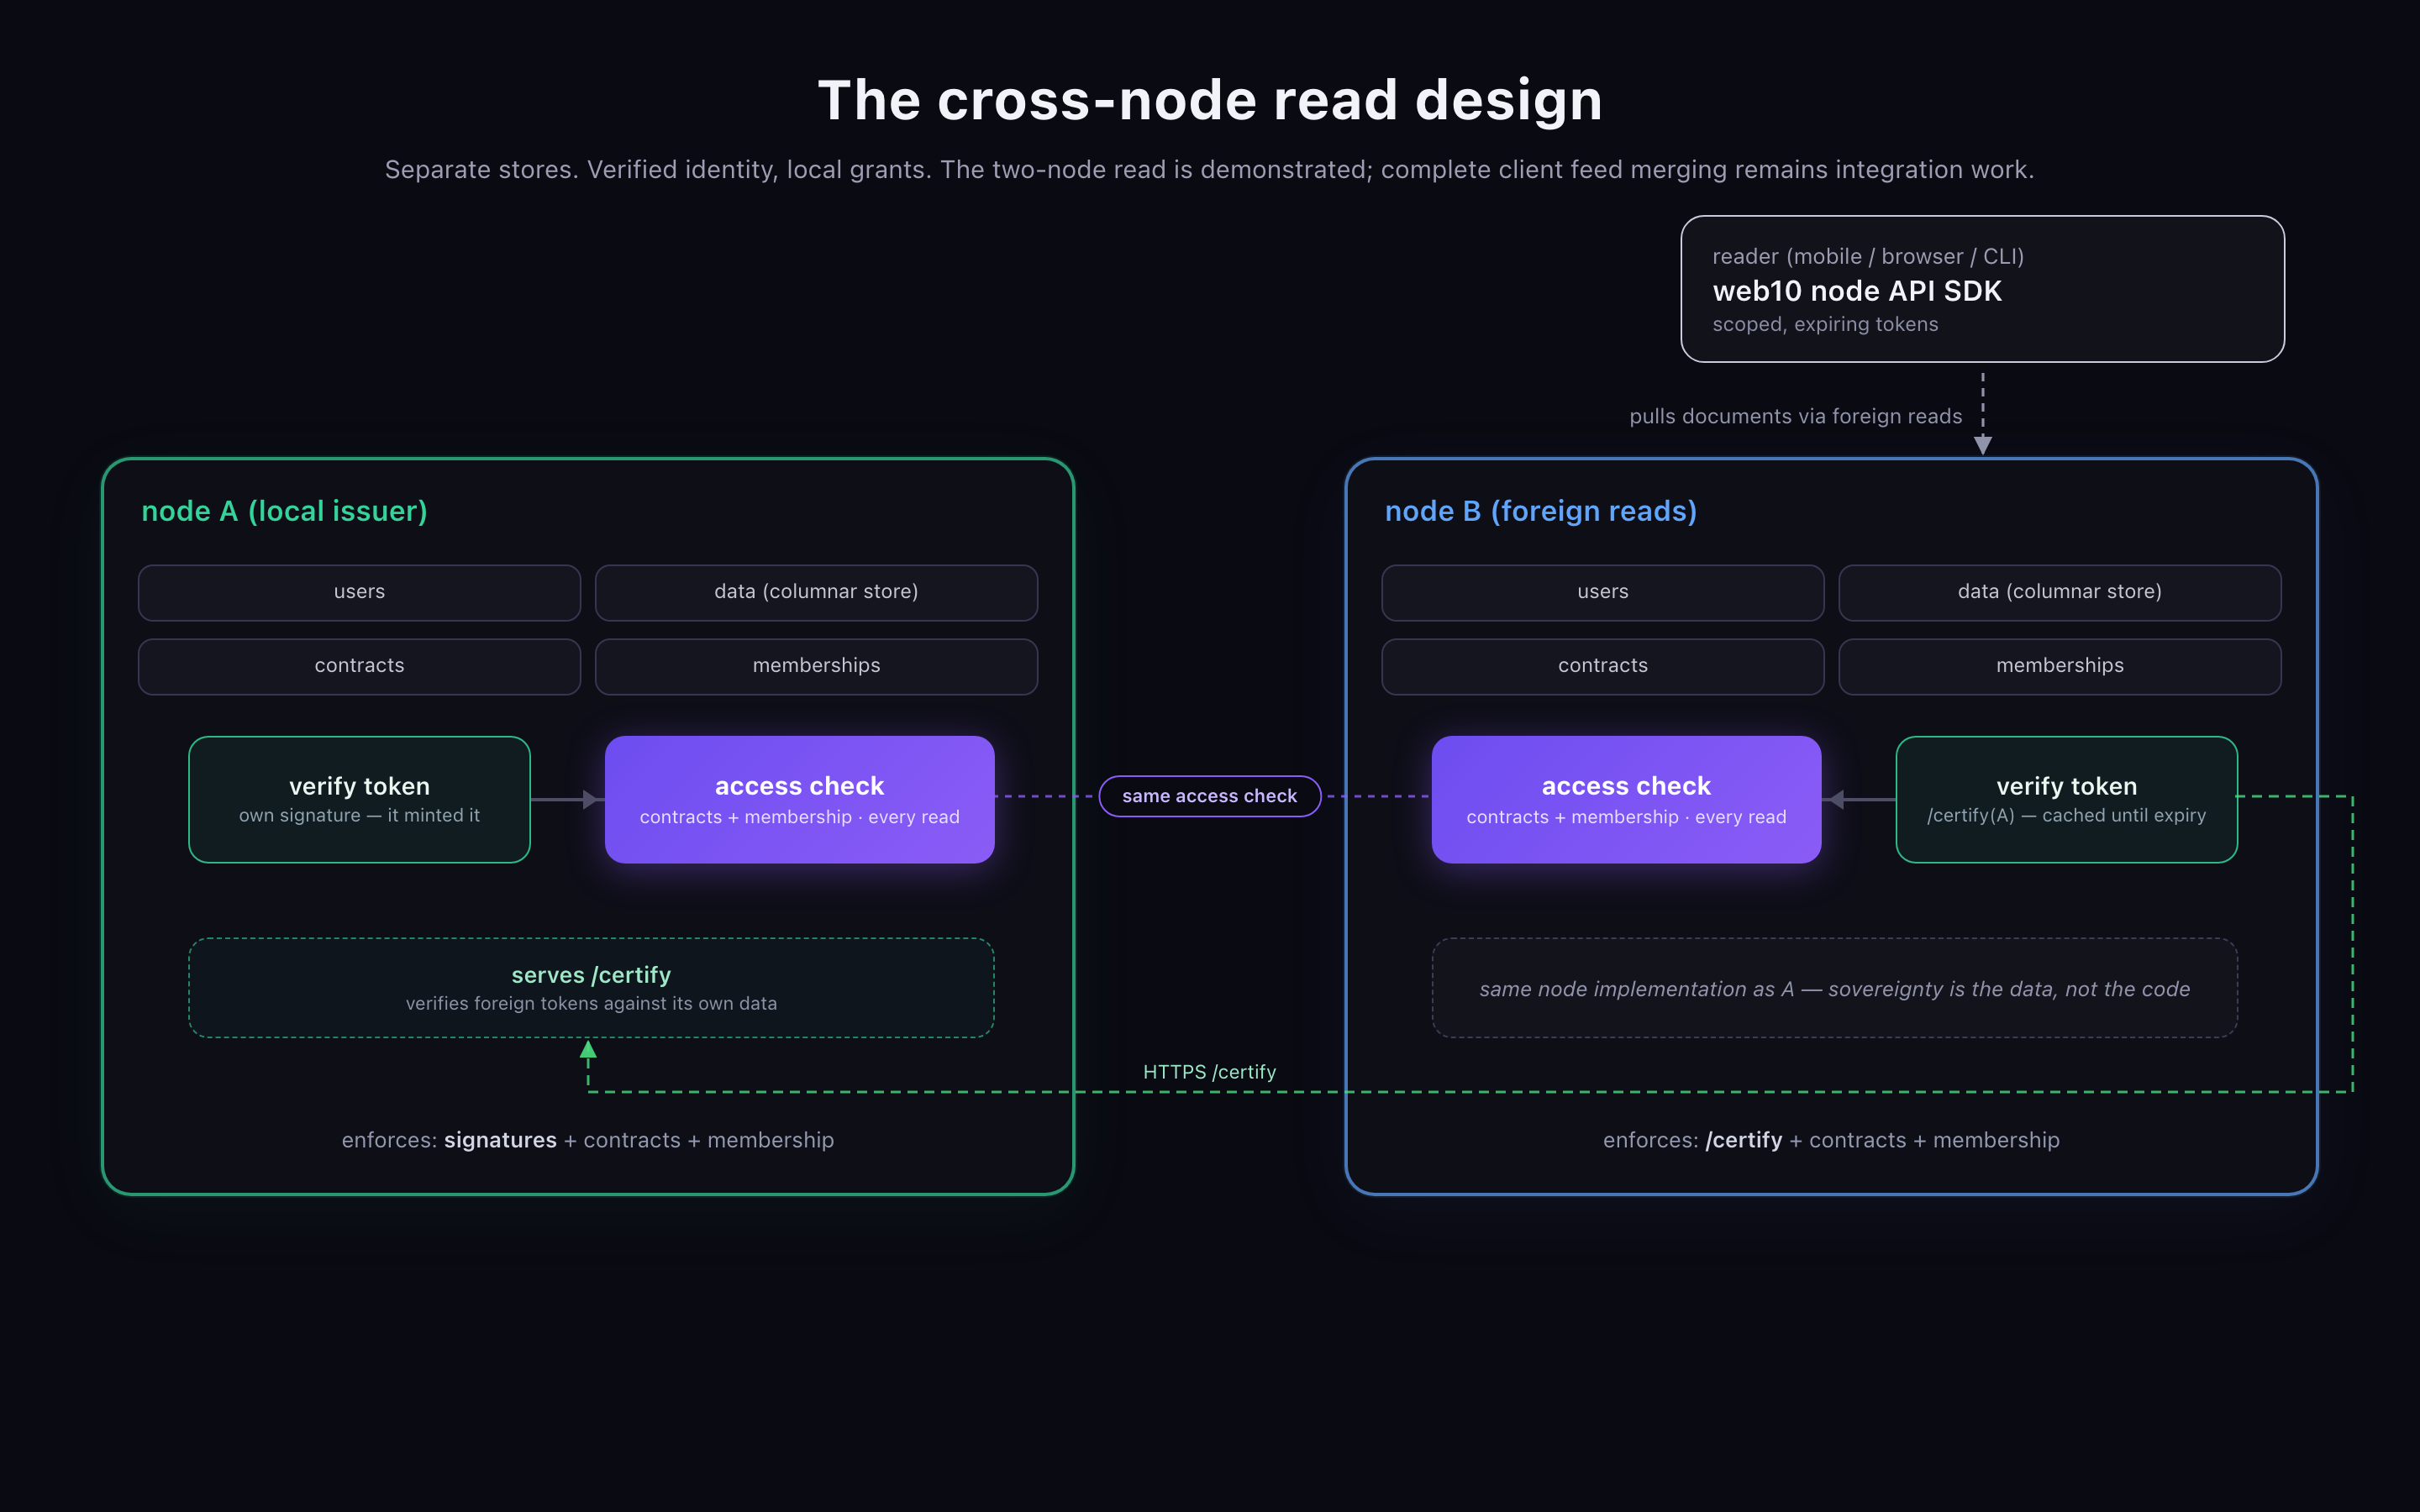
\includegraphics[width=\textwidth]{figs/fig-feed.png}
\caption{Cross-node read design: certify identity, then apply local grants.}
\label{fig:feed}
\end{figure*}

\subsection{A public subscription that outlives an account}
\label{sec:domain}

An account principal and a public address serve different purposes.
The domain prototype uses a creator-controlled domain as the public
address. A TXT record at \texttt{web10.\emph{domain}} names its target:
\texttt{web10.v=1; provider=\emph{node}; user=\emph{username}}.
The creator authenticates to the target node and calls
\texttt{POST /v3/domains/verify}. The node performs the DNS lookup itself
and checks that the record names this node and this account before
storing a verified alias. DNS discovers the account; it does not replace
the account's authentication or group principal.

The reader stores the domain in a private document at the reader's home.
On a later read, the prototype resolves that domain, checks the target's
verified alias, and requests public content. When the creator changes
provider, the creator changes the TXT pointer and verifies the new
account. The saved subscription does not change. The old node cannot
edit a DNS zone the creator controls, and the move need not ask the old
node to release its stored alias.

Figure~\ref{fig:audience-portability} follows this indirection through a
provider change. The fan's subscription remains in the fan's data;
the creator changes the address's target. Neither old content nor private
grants are transferred by DNS. The demonstrated benefit is continuity of
\emph{public discovery}, not continuity of private authority. The
research client implements this behavior; production social follows are
unchanged. It assumes retained domain control and available DNS, reader
home, and replacement provider. Domain expiry or theft can redirect
the subscription.

\begin{figure*}[t]
\centering
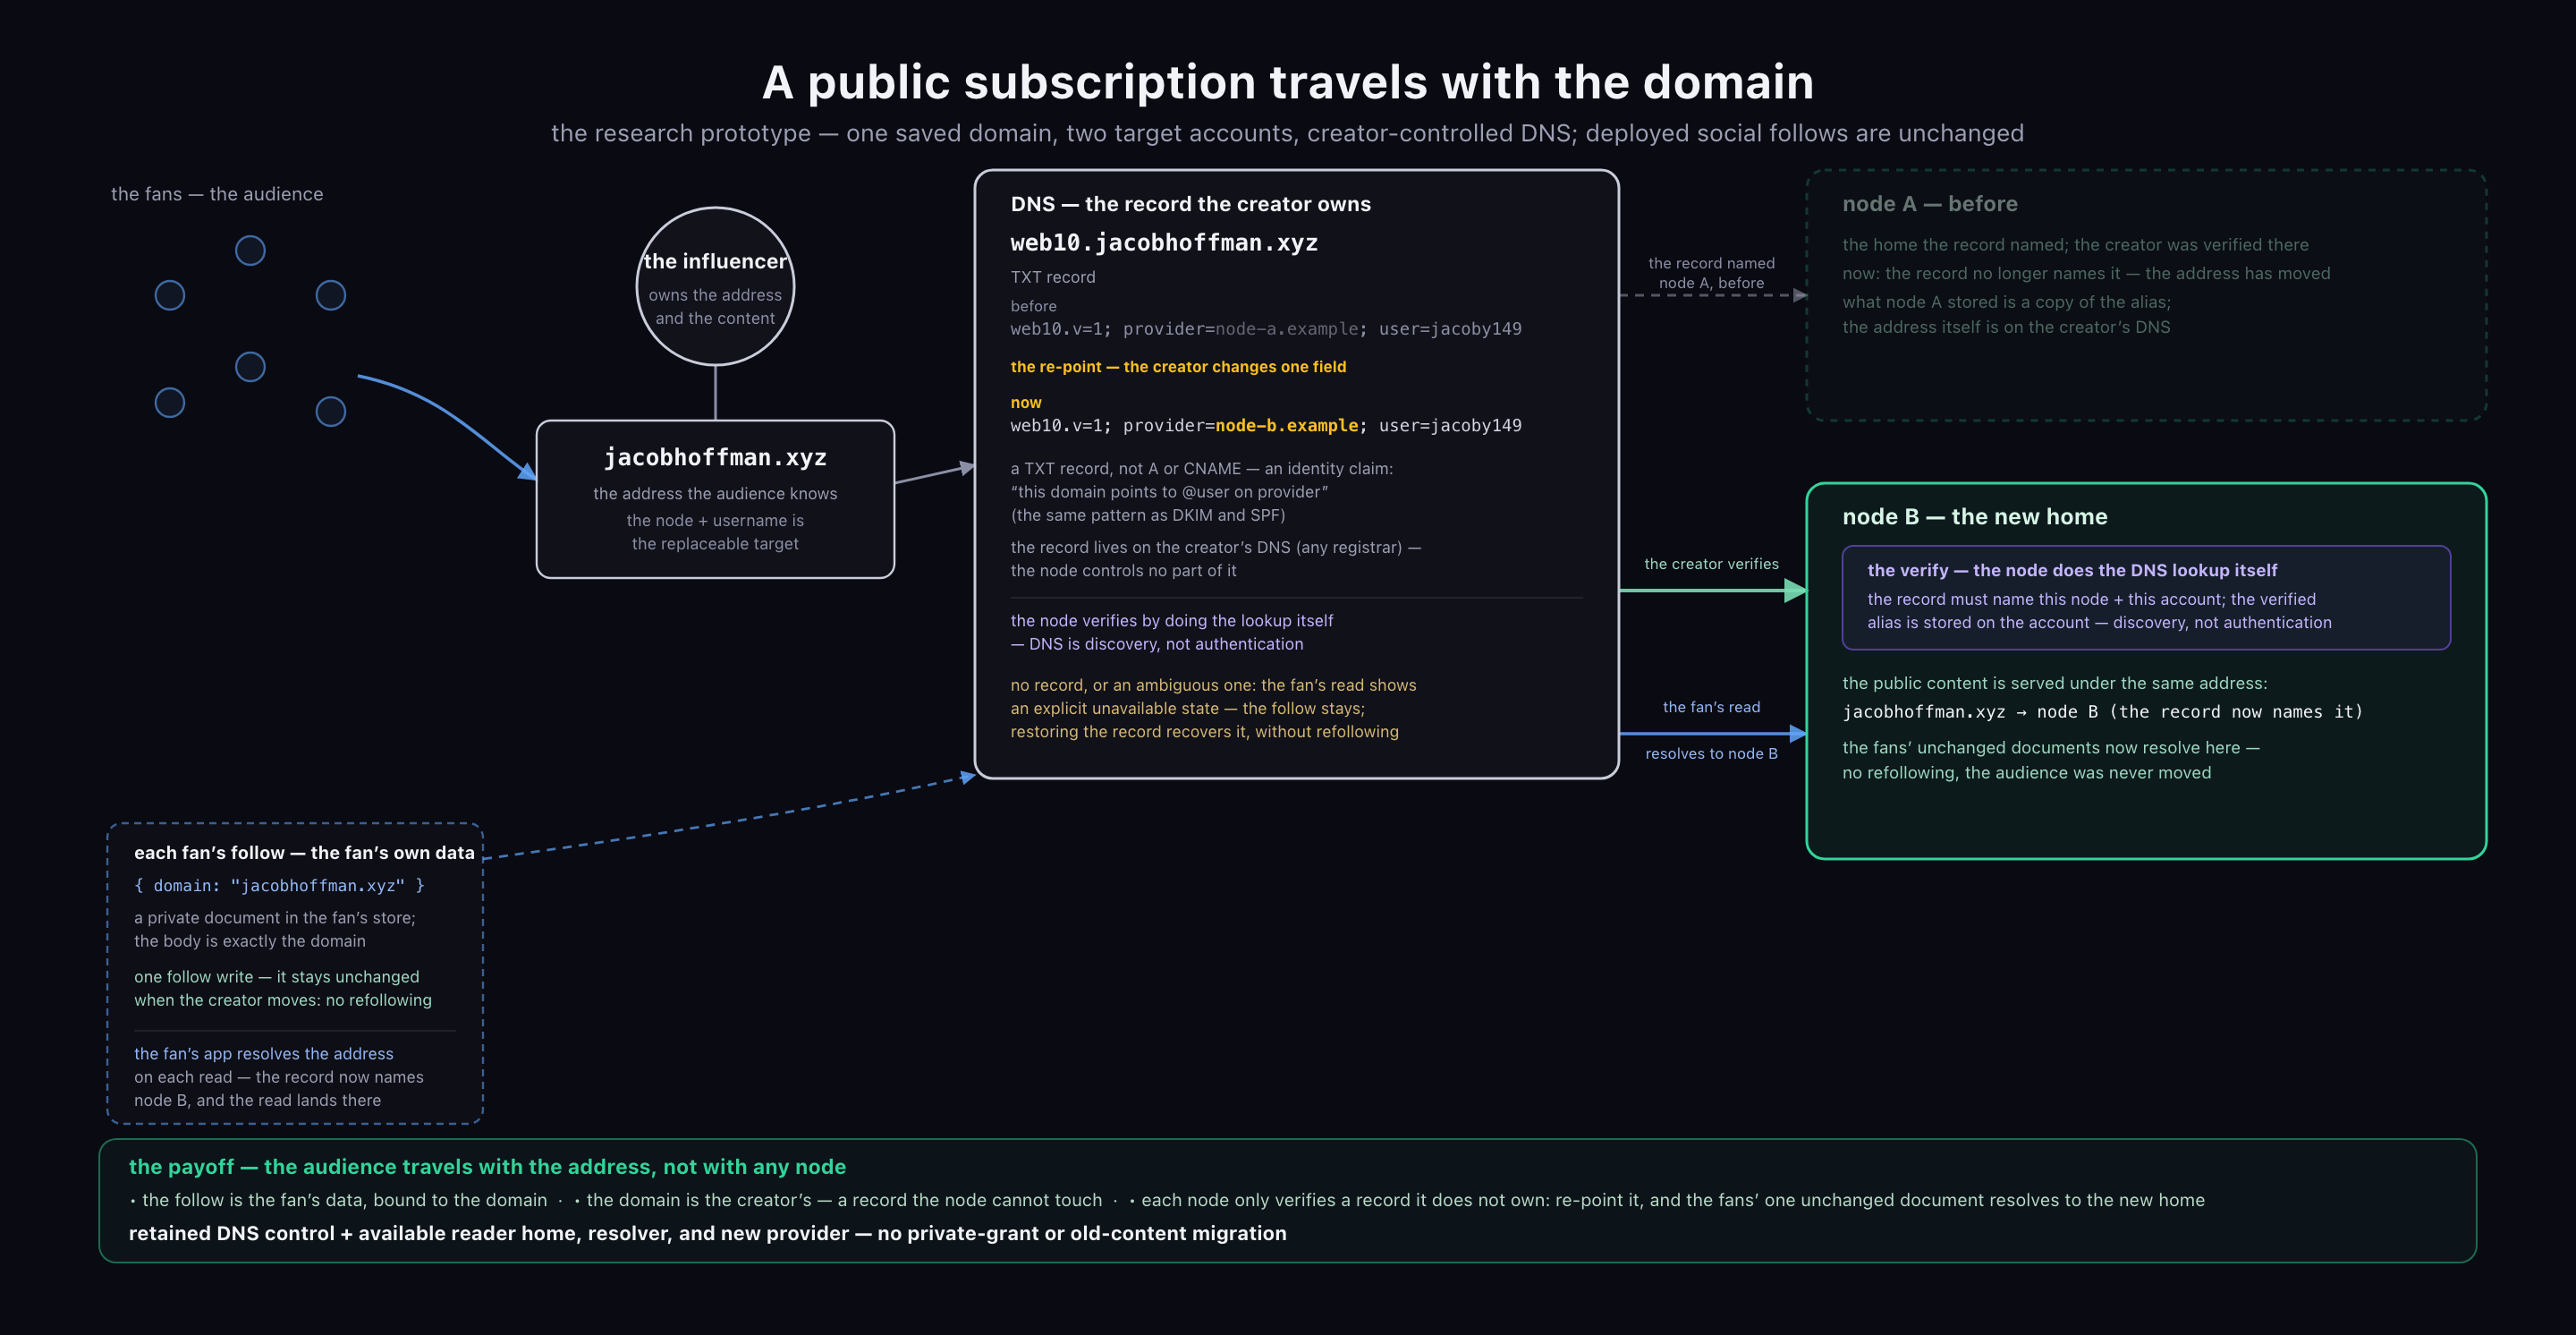
\includegraphics[width=\textwidth]{figs/fig-audience-portability.png}
\caption{The domain-follow prototype: a new target, the same subscription.}
\label{fig:audience-portability}
\end{figure*}

\section{Advertising without owning the creator's payout}
\label{sec:money}

A creator platform also needs an economic model. web10's current
approach is an advertising rail, not a payment processor. A creator's
offer is data: the creative, offer kind, destination link, call to
action, and disclosure. Affiliate and sponsor payments settle outside
the node. web10 does not rewrite the creator's link or take a percentage
of those payouts. This is a policy of this rail, not a claim that
creators cannot monetize on other decentralized systems.

The rail separates a creator's pinned offer from the node operator's
overlay. Result preparation can attach both to one
document; the node's overlay does not replace the creator's offer.
The operator configures overlay density, with a default of 10\%.
Selection is deterministic per reader and inventory rotation distributes
the selected node ads. Ad documents remain subject to their own access
checks; an authorized post is not blanket authority to read any creative.

Creators choose pinned offers; operators configure their own inventory.
Creator payouts, operator advertising revenue, and hosting fees are
distinct. No revenue share, exposure target, or market outcome is measured.
web10-social builds the catalog; Snake and Marketplace do not demonstrate
ad rendering. An exchange and payment processing remain future work.

\section{Lessons from building and operating the node}
\label{sec:lessons}

\subsection{Generality has to survive the primary application}

The social application repeatedly created pressure for bespoke node
features. Four were built and then removed: a dedicated feed endpoint,
a group-identity table and endpoint, a followers-group check in the
session oracle, and an ad path hard-coded to a collection name. Their
replacements were, respectively, an application query, documents in an
app-named service, application-side session logic, and generic tags and
group attachments.

The test was practical: would a notes application, music application,
or shop use this node operation? If not, the concept belonged in the
application. Holding this line moved more orchestration into the browser.
It also made the later game and marketplace possible without extending
the node for either of them. The generic core emerged from removing
plausible shortcuts, not from keeping the first design untouched.
Ad preparation and Discover still require a separate genericity review;
the removed shortcuts do not establish project-wide compliance.

\subsection{A schema repair is not ready until readers can use it}

The connected interoperability work encountered a fresh-stack failure:
\texttt{group\_contracts.tags} was absent when an early request needed
it. The runner had launched the API before initializing the database.
Starting storage, initializing schema, and then starting the API let the
existing boot migration operate against real tables. This was a runner
ordering repair, not closure of the project-wide fresh-start issue.

The general requirement is stronger than eventually adding a column:
required schema must exist before readers are admitted. A fresh database
and its first request need a separate test from the steady-state system.
Deferring an upgrade is safe only when no admitted request depends on it.

\subsection{A shared analytical engine still pays operational costs}

\texttt{ReplacingMergeTree} removes obsolete versions during background
merges, but reads cannot wait for those merges to establish correctness.
They resolve versions explicitly. Tombstones participate in that ranking;
they cannot be filtered away first. Documents attached to multiple readable
groups also create join multiplicity, so applications must choose the
deduplication semantics of counts and pagination.

The same shared engine handles metadata lookups and analytical scans.
Merge work consumes resources, small point queries pay fixed round-trip
costs, and tenants share the node's capacity. Query freedom therefore
creates an operational obligation to manage resource use. The first
fan-out measurement found a bottleneck in repeated permission-metadata
queries rather than document scanning. Reducing those round trips was
more valuable for that workload than changing its document query.

\section{Evidence}
\label{sec:evaluation}

The evaluation answers four mechanism questions and reports one deployed
operating point. The mechanism experiments use synthetic data on isolated
stacks. The operating point is a read-only production observation. None
of these is a concurrent-capacity trial or a performance comparison
against another platform.

\subsection{Can another application reuse social-written data?}
\label{sec:ev-interop}

In the browser scenario, a fresh user logged into web10-social through
its authenticator popup and changed the profile name to Alex Morgan.
The user approved Snake's service request, earned and saved ten points,
and saw the joined social identity on the leaderboard. Revoking the app
contract made a new query return 403; the leaderboard cleared the result
and displayed an access error. After sign-out, Marketplace requested
its permission through the popup, published a listing, and showed the
same social-written identity. Reloading the detail URL retained the
correct listing. API assertions compared profile bodies, authors, counts,
and document identifiers, so a username fallback could not pass.
The reused profile is written by the actual social application, not a
separate mock profile store built just for the game and marketplace.

A separate three-account HTTP case checked exact two-author score/profile
and listing/profile joins. Missing application permission for
\texttt{profile} denied the queries; granting it enabled them; revocation
denied them again. A separately labeled private-profile fixture tested
the group gate: membership enabled the inner join, and removal emptied
that join while scores remained readable.

The final fresh-stack run on 2 November 2026 passed desktop (1440 pixels),
mobile (375 pixels), and HTTP correctness: three cases, zero retries,
zero skips. The host was a four-vCPU, 8-GB DigitalOcean sfo2 instance
running ClickHouse 24.8.14.39; browser tooling used Playwright 1.63.0 and
Chrome for Testing 153. The \evidence{research/interoperability-demo}{artifact}
retains the exact base-plus-patch source, overlay, configurations, image
identities, outcomes, and 16 captures.

Both demos share a browser origin and profile convention; the HTTP control
supplies a distinct application Origin. These are consent, reuse, and
revocation results, not independent adoption (\S\ref{sec:limitations}).

\subsection{Can a foreign principal read, lose access, and read again?}
\label{sec:ev-network}

Two API processes used separate ClickHouse and MinIO instances and
independently generated HS256 signing secrets. The serving node reached
the home issuer through real HTTPS with an ephemeral test CA and issuer
hostname verification. Bob created a private group and document on B.
Alice's A-issued token was denied on B's document and query paths.
Granting membership to B's distinct, same-named Alice still denied
A's Alice. Granting the exact foreign principal enabled both reads of
the exact document; removal denied both; regrant restored both.

All lifecycle reads reused the same JWT. The issuer recorded one
successful certification across that lifecycle, while B reapplied access
checks on every request. A forged foreign-provider token signed with
B's key was rejected; repeating it used a negative cache entry rather
than another issuer call. A separate Origin-bearing query control
returned 403, 200, and 403 around a qualified foreign app-contract grant
and revocation. Its app-contract setup was a service-function fixture,
not browser consent.

The unchanged scenario passed on clean merged source with an empty
patch. The \evidence{research/federation-demo}{artifact} retains the
source identity, 34 status events, configuration, image identities,
issuer traffic, and verified cleanup. Docker-internal addressing and a
test CA bound this correctness slice; deployment and revocation limits
are collected in \S\ref{sec:limitations}.

\subsection{Can a public subscription survive the old provider's loss?}
\label{sec:ev-domain}

The separate domain client stored the creator's normalized domain in a
private \texttt{domain-demo-follows} document at the reader's home.
On desktop (1440\,$\times$\,1000) and mobile (375\,$\times$\,812), the
creator published a TXT record and verified the old account through
actual local UDP DNS. The reader clicked Follow once and read its
public post. The harness then stopped the old API and TLS frontend.

The creator pointed DNS to a new account and verified it without
contacting the old provider. Reader reload and ordinary login displayed
the new account's public content with the identical saved follow ID and
body and exactly one follow creation. No old content was migrated.
The independent private controls returned 200 for the explicitly granted
old private source and 403 for the new target's private content. The
public pointer did not transfer private authority.

Missing or ambiguous DNS cleared displayed content without removing
the subscription. Restoring DNS recovered it without refollowing.
Delayed real responses at five identity-transition boundaries verified
that logout and account changes prevented stale UI updates. DNS, alias,
and public-content requests carried no credentials. The
\evidence{research/domain-portability-demo}{artifact} retains the clean
committed integration, exact inputs, ten captures, request outcomes,
and cleanup.

The result is public-subscription continuity in two configured lab
origins, under the availability, DNS, and domain-control fixtures
collected in \S\ref{sec:limitations}; it is not production integration.

\subsection{Where does readable-group resolution become expensive?}
\label{sec:ev-cost}

The query path resolves readable groups before executing the application's
relational operations. The experiment varies candidate-group count
$K$ to compare point metadata lookups with batched resolution.
Figure~\ref{fig:k1000-curve} plots readable-group time, not browser
latency or complete feed assembly.

\textbf{Historical setup.} One sequential trial ran in DigitalOcean sfo2;
no independent repeat or paired authorization baseline is available here.
The \texttt{s-4vcpu-8gb} host provided four vCPUs and 8\,GB nominal RAM.
It ran Ubuntu 24.04, Linux 6.8, and Docker 29.1.3, with one Uvicorn
process and ClickHouse 24.3.18.7.
Seed 42 created 1,000 creators with one small post each and a reader who
joined all their groups. Those groups also permitted public reads.
Personal queries supplied $K=10$, $100$, and $1{,}000$ on this same
dataset. A separate discover query used one board group and ten
additional posts. Twenty samples in each of 20 cells produced 400
measurements: 320 HTTP requests and 80 direct engine executions.
All HTTP requests returned 200.

\textbf{Variants.} The per-group resolver issues point metadata queries.
The batched resolver fetches memberships, principal-class grants, and
role definitions in three queries, then resolves access in memory.
Variant B executes the real document query. Variant C substitutes a
fixed 20-row scan result while retaining policy resolution and
compilation. Variant A precompiles the known-readable projection and
times execution directly in ClickHouse outside the HTTP handler.

The document query selects IDs and bodies, orders by creation time and
ID, and limits to 20 rows. It omits engagement joins, media preparation,
and browser assembly. HTTP requests omit Origin and do not exercise the
browser-origin app-contract gate. C is not an output-equivalent
execution, and A excludes authentication, compilation, and serialization.

\textbf{Finding.} Table~\ref{tab:fanout} reports all B cells.
From $K=10$ to $1{,}000$, median readable time grew $100.44\times$
per-group and $9.12\times$ batched. At $K=1{,}000$, batching reduced
median handler time from 7,644.66\,ms to 363.31\,ms ($21.04\times$)
and readable time from 7,535.71\,ms to 213.98\,ms ($35.22\times$).

Stubbing document execution preserved the separation: at $K=1{,}000$,
C's readable medians were 8,388.39\,ms per-group and 222.57\,ms batched.
A's direct execution medians ranged from 28.6\,ms to 54.2\,ms across the
personal queries. Repeated metadata work, rather than the simplified
document scan, dominated the unbatched path. The result supports using
the batched resolver for large candidate sets. The endpoint default
remains per-group; this draft contains no deployed-default repeat.

\textbf{Tradeoff.} On the one-group discover query, per-group resolution
was faster: 9.53\,ms readable versus 25.37\,ms batched. The three fixed
round trips cost more than a small number of point checks. Batching also
did not make cost constant: batched median handler time grew
$4.47\times$ across the 100-fold increase in $K$.

The trial had no concurrency sweep, randomized cell order, or explicit
warm-up exclusion. Twenty samples yield preliminary within-run
percentiles, not independent repeated-trial characterization. The
\evidence{research/experiments/costfn}{artifact} retains the setup,
source, report, and per-cell summary receipts; it does not retain all
raw per-sample measurements. Success statuses alone do not establish
permission equivalence across policies. $B-A$ is a pipeline-versus-scan
comparison, not a causal authorization-overhead estimate. An earlier
100-creator trial used a different host and snapshot and is not pooled
with this one.

\begin{figure*}[t]
\centering
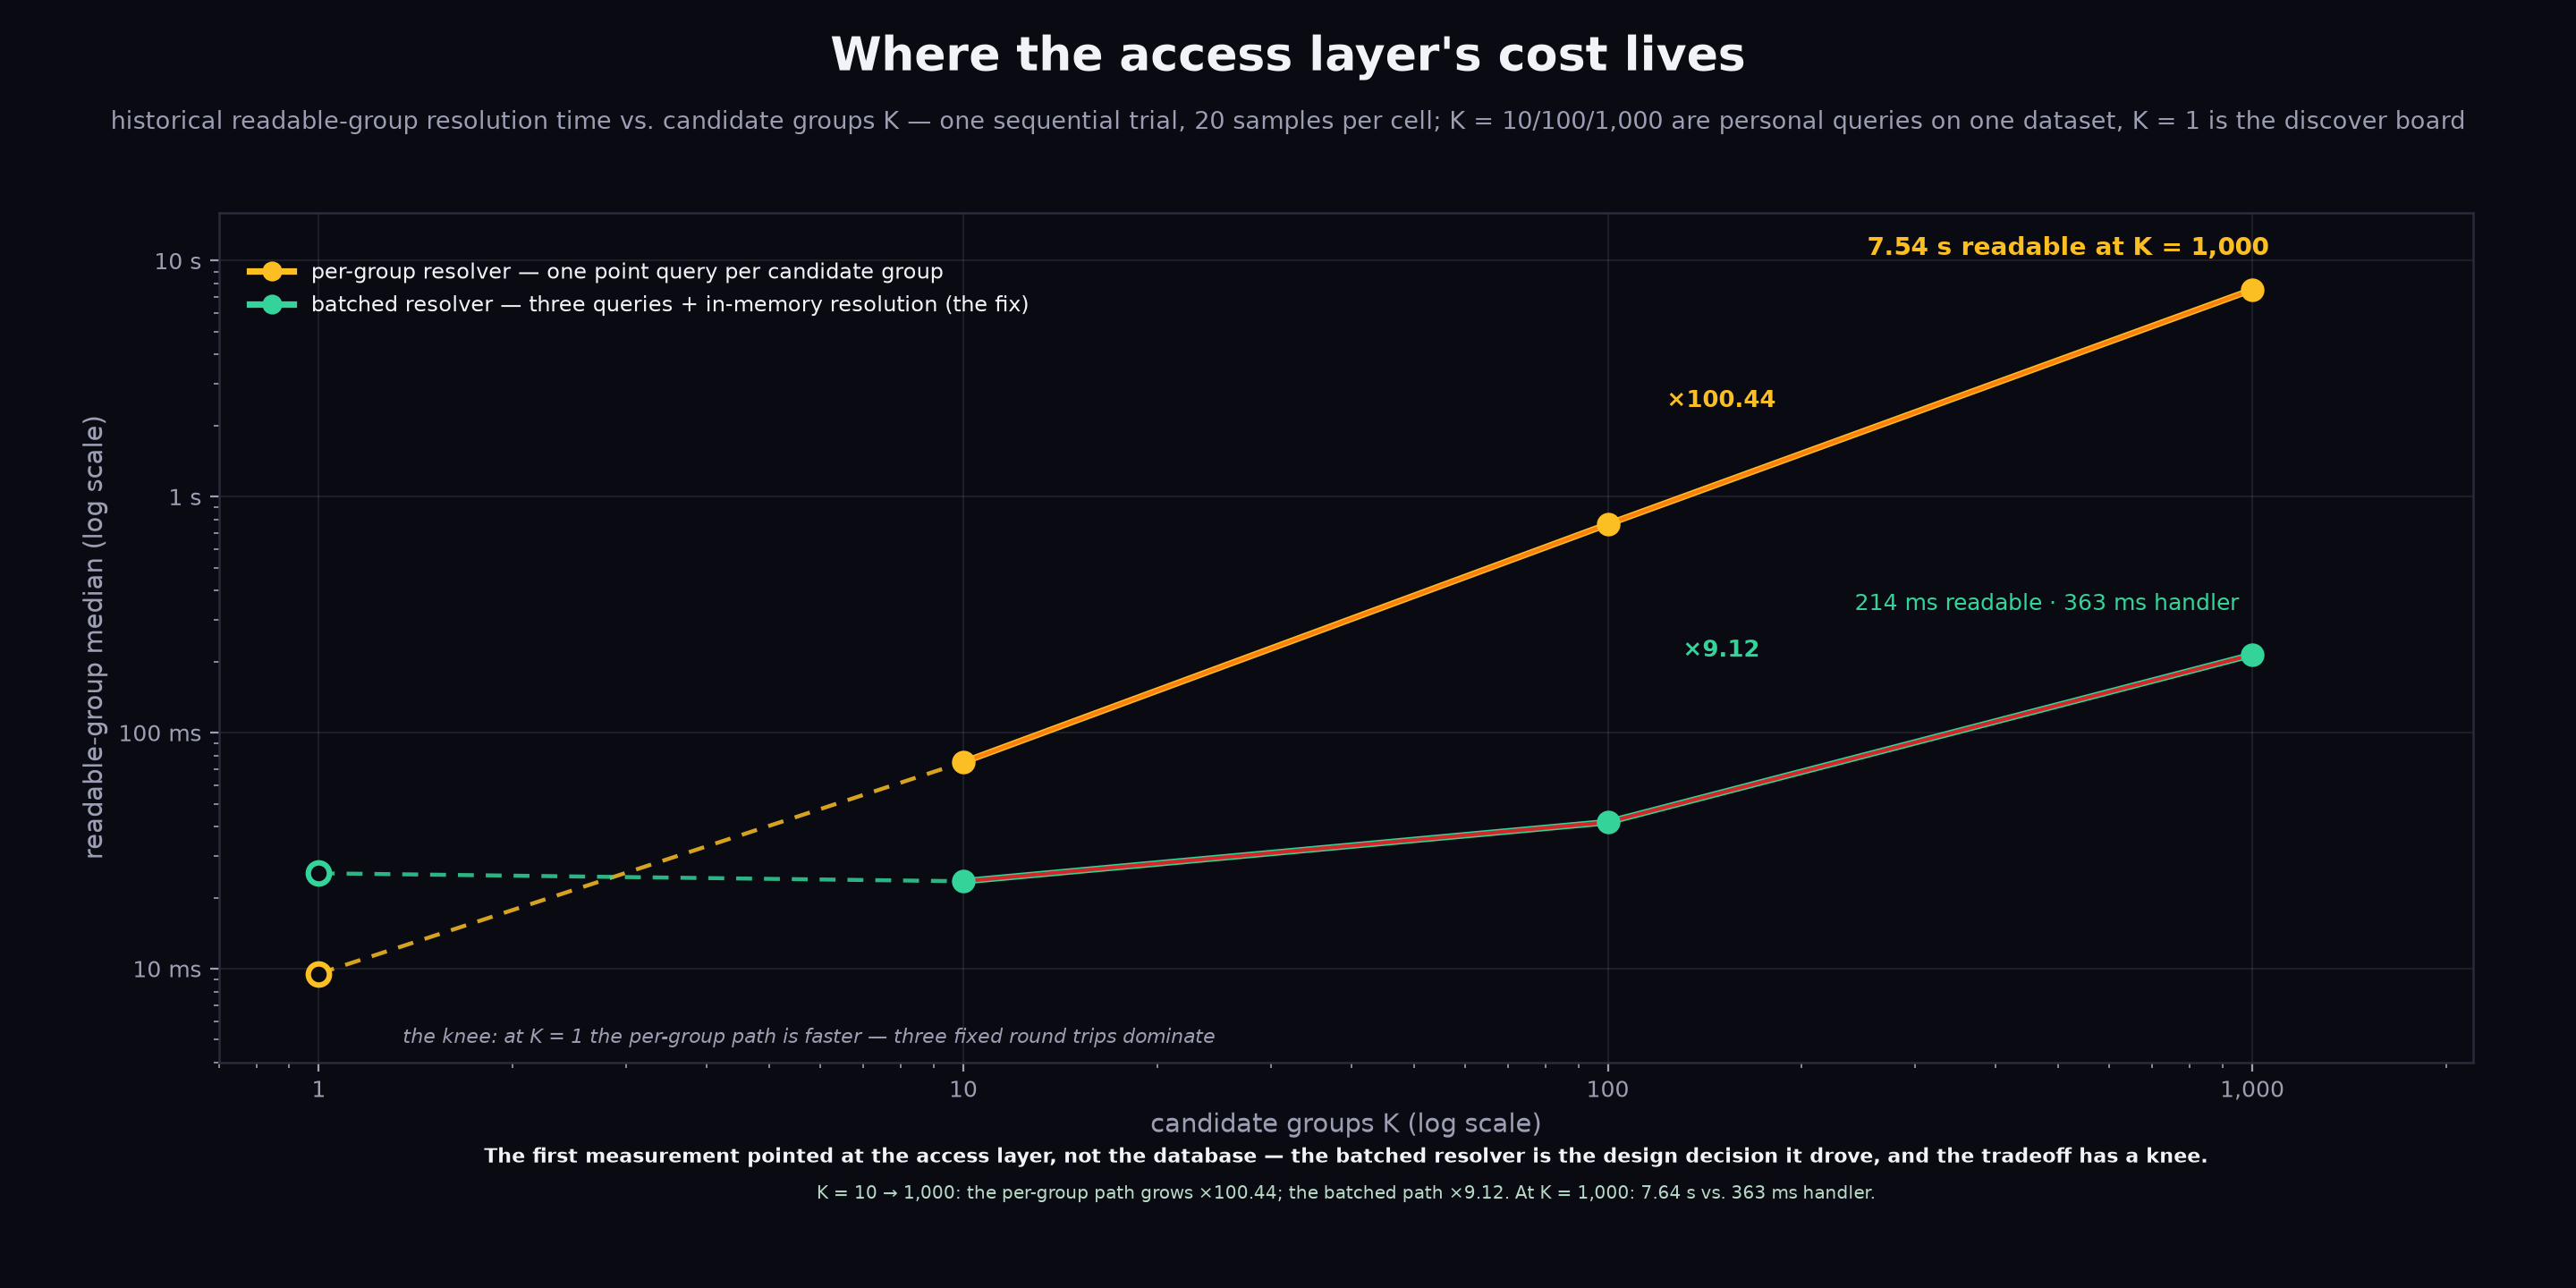
\includegraphics[width=\textwidth]{figs/fig-k1000-curve.png}
\caption{Readable-group resolution cost and its small-$K$ tradeoff.}
\label{fig:k1000-curve}
\end{figure*}

\begin{table}[t]
\centering
\caption{Historical B trial: handler and readable-resolution latency (ms).}
\label{tab:fanout}
\small
\setlength{\tabcolsep}{3pt}
\begin{tabular}{rlrr}
\toprule
$K$ & Resolver & Handler p50 / p95 & Readable p50 / p95 \\
\midrule
10 & per-group & 129.355 / 171.177 & 75.030 / 93.295 \\
10 & batched & 81.275 / 98.907 & 23.470 / 31.174 \\
100 & per-group & 831.350 / 915.175 & 764.385 / 843.210 \\
100 & batched & 99.415 / 139.469 & 41.775 / 51.651 \\
1,000 & per-group & 7,644.655 / 8,679.235 & 7,535.705 / 8,504.610 \\
1,000 & batched & 363.305 / 435.028 & 213.980 / 284.032 \\
\bottomrule
\end{tabular}
\end{table}

\textbf{Proposed load target, not results.} Table~\ref{tab:funnel} makes
the million-user sizing assumptions explicit. With one session per DAU,
concurrent users equal peak-hour sessions times session minutes divided
by 60, including idle time. The proposed seed is one million registered
authors with one post each, not one million measured active users.
At 10,000 concurrent users and 60-second feed think time, the offered
load is about 167 feed loads/s: 500 query calls/s plus 167 content-views
requests/s before auxiliary work. At 30 seconds these rates double.
In-flight requests equal request rate times latency, not concurrent users.
Stepped trials at 1k/3k/5k/10k/20k virtual users, raw samples, repeated
runs, errors, throughput, p50/p95/p99, and host utilization remain open.

\begin{table*}[t]
\centering
\caption{Proposed million-user funnel; assumptions, not observed load.}
\label{tab:funnel}
\begin{tabular}{llrrrr}
\toprule
Scenario & Population definition & DAU & Peak share & Sessions/h & Concurrent (5 / 15 min) \\
\midrule
Low & 1M registered; 300k MAU & 100k & 12\% & 12,000 & 1,000 / 3,000 \\
Likely & 1M MAU & 250k & 15\% & 37,500 & 3,125 / 9,375 \\
High & 1M MAU & 500k & 15\% & 75,000 & 6,250 / 18,750 \\
\bottomrule
\end{tabular}
\end{table*}

\subsection{What does the deployed operating point show?}
\label{sec:ev-production}

A read-only production observation on 28 October 2026 recorded 597
account rows, 593 live documents across 30 distinct authors and ten
services, 49 group contracts, and 1,298 membership rows. Nine
authenticated browser navigations across following feed, music, and
groups returned HTTP 200, retained the session, and produced no uncaught
page errors. The following feed rendered 20 posts in a median 5,396\,ms
of full-page readiness.

This dated operating point establishes deployment and observed use,
not a large active-user population or capacity bound. The host also ran
a development stack; the snapshot has no activity window. Full-page
readiness includes frontend startup and network work and is not the
query-handler time measured above. The 5.4-second result makes the next
measurement concrete: dissect complete page assembly, including
follow-up engagement reads and media delivery, rather than extrapolating
from the simplified query.

\section{Positioning the combination}
\label{sec:related}

\textbf{User-controlled storage and interoperable records.}
Solid~\cite{solid2016,solid-apps2016,css2024} is the closest antecedent
for separating applications from user-controlled storage. WAC supports
resource access and group agents; ACP includes agent, client, and issuer
matching~\cite{wac2022,acp2022}. web10 does not introduce user-managed
authorization into an otherwise permissionless field. It combines
service/group grants with a shared, node-hosted SQL interface. The
comparison in Figure~\ref{fig:composition} is pod fetching or an added
index versus shared-store queries; millions is sizing, not measured capacity.

ActivityPub defines federated activity exchange~\cite{activitypub2018}.
AT Protocol separates repositories, relays, and AppViews and supports
extensible Lexicons~\cite{kleppmann2024}. Its current permissions
specification scopes public-repository writes by collection and action
and supports remote-service RPC permissions~\cite{at-permissions}.
These are substantial forms of extensibility and delegation. The
Statusphere example also shows how application-owned synchronization
and database queries construct a new cross-user view~\cite{at-statusphere}.
web10 supplies the shared query service at the storage node and includes
group-controlled private document access in that same substrate. This
can reduce infrastructure for an application needing those operations;
it also places query execution and resource contention at the node.

\textbf{Authorization and shared databases.}
User-specific grants and reader-filtered relations are established
ideas. Multi-tenant systems have long shared tables under logical
tenant identifiers~\cite{force2009,aulbach2008,jacobs2007}.
PostgreSQL policies place row access inside query execution
\cite{postgres-rls}. Zanzibar addresses relationship-based authorization
and consistency across services~\cite{zanzibar2019}, while TAO provides
an operational precedent for social-graph storage and read-time privacy
checks~\cite{tao2013}. web10 joins these concerns in a different
deployment unit: end-user data and grant metadata in one columnar
database, with application queries compiled against authorized service
relations. It does not claim Zanzibar's consistency guarantees or a
measured advantage over an equivalent engine-level policy.

\textbf{The contribution.} The system contribution is this integration,
demonstrated through cross-application reuse and isolated cross-node
authorization, with a measured metadata fan-out tradeoff. The advertising
rail is an application of the substrate, not evidence that other
decentralized protocols prohibit creator revenue. Building the primary
social app ourselves makes the substrate answer to an actual consumer;
it does not establish independent-developer adoption.

\section{Limitations}
\label{sec:limitations}

\textbf{Evaluation.} One dated operating point, synthetic correctness
slices, and one sequential fan-out trial are not a production load test.
The trial retains summaries, not raw samples; cell order is not randomized,
warm-up is not excluded, and p95s are preliminary. It omits engagement,
media, browser assembly, and the Origin gate. The default remains per-group;
deployed-batched repeats, a paired same-engine ablation, million-author
load, and concurrency remain unmeasured. The October snapshot shares a
development host and has no activity window. A nonempty feed needs three
queries plus content views and possible author resolution, not the
benchmark's single query.

\textbf{Genericity and isolation.} Apps author ranking; ClickHouse executes
it. Node-supplied ad loaders and Discover directory/enrollment leave the
genericity audit open. Interop shares browser origin and conventions;
HTTP Origin controls prove neither separate-origin browser isolation nor
independent adoption. Media and revocation latency are unmeasured;
parser/media correctness needs broader review, not an AST-only safety claim.

\textbf{Network.} Two-process Docker-internal federation uses a test CA and
fixture grants, not public deployment or browser consent. Principal
migration, foreign self-join, production keys, multiworker/restart behavior,
feed merging, and issuer revocation bounds remain open. The two-origin
domain prototype uses TTL-zero local DNS, a loopback bridge, certificate
exceptions, and app/private-grant fixtures. It proves neither content/private
authority migration, production follows, public-DNS timing, arbitrary
onboarding, nor absolute unbannability; domain control and service
availability remain assumptions. Advertising exposure, revenue, and
game/marketplace rendering are unmeasured.

\section{Conclusion}
\label{sec:conclusion}

Our social app, game, and marketplace exercise authorized node-side computation.

Isolated network slices separate identity from grants and public continuity
from private authority, not production integration or migration.

The historical trial found 7.64\,s versus 363\,ms handler time at 1,000
groups, with a cost at one group. Independent repeats, full-feed/concurrent
workloads, and a paired same-ClickHouse pre-authorized baseline with
equivalent rows/order remain open. So do production cross-node integration,
revocation bounds, and broader parser/media correctness.

The contribution is the combination: user-managed access and
application-defined computation on the same shared columnar store,
exercised by our social app and cross-app profile reuse. Solid fetches pods
or adds an index; millions remains unmeasured sizing. AT's alternative
backend is possible but costs infrastructure.

\bibliographystyle{ACM-Reference-Format}
\bibliography{web10-references,comparisons}
\end{document}
